\documentclass[lettersize, journal]{IEEEtran}

\usepackage{hyperref}
\usepackage{url}
\usepackage{float}
\usepackage{amsmath}
\usepackage{graphicx}
\usepackage{color}
% \usepackage[style=numeric]{biblatex}
% \addbibresource{references.bib}
\usepackage{multirow}
\usepackage{makecell}
\usepackage{threeparttable}
\usepackage{algorithm}
\usepackage{algorithmic}
\usepackage{bm}
\usepackage{ulem}
\usepackage{mathtools, nccmath}
\DeclarePairedDelimiter\floor{\lfloor}{\rfloor}

\renewcommand{\thefootnote}{\fnsymbol{footnote}}

% \usepackage[nodisplayskipstretch]{setspace}
% \setstretch{1.5}

% \setlength{\intextsep}{1pt}
% \setlength{\textfloatsep}{1pt}
% \setlength{\abovecaptionskip}{1pt}
% \setlength{\belowcaptionskip}{1pt}

% \makeatletter
% \setlength{\@fptop}{3pt}
% \makeatother

\newcommand\hiddenref[1]{\sbox0{\cite{#1}}}
\usepackage{amsmath,amsfonts}
\usepackage{algorithmic}
\usepackage{algorithm}
\usepackage{array}
\usepackage[caption=false,font=scriptsize,labelfont=sf,textfont=sf]{subfig}
\usepackage{textcomp}
\usepackage{stfloats}
\usepackage{url}
\usepackage{verbatim}
\usepackage{graphicx}
\hyphenation{op-tical net-works semi-conduc-tor IEEE-Xplore}
% updated with editorial comments 8/9/2021
% \raggedbottom


\begin{document}

\title{Finger-Knuckle Assisted Slap Fingerprint Identification System for Higher Security and Convenience}

% \author{Zhenyu Zhou, Ajay Kumar,~\IEEEmembership{Fellow,~IEEE}}
\author{{Zhenyu Zhou, Ajay Kumar}

% \thanks{This paper was produced by the IEEE Publication Technology Group. They are in Piscataway, NJ.}% <-this % stops a space
\thanks{Authors are with the Department of Computing, The Hong Kong Polytechnic University, Hung Hom, Kowloon, Hong Kong.}}

% The paper headers
\markboth{Journal of \LaTeX\ Class Files,~Vol.~x, No.~x, ~2022}%
{Shell \MakeLowercase{\textit{et al.}}: A Sample Article Using IEEEtran.cls for IEEE Journals}

\maketitle

\begin{abstract}
  Billions of fingerprint images are routinely acquired to support e-governance programs and protect national borders using millions of slap-fingerprint acquisition devices that are deployed globally. Several studies from national ID programs like UIDAI \cite{uidai}, and NIST \cite{2002SUMMARYON}, have indicated that ~2\% of the user population may not have usable fingerprints. Finger knuckle patterns are inherently presented during such slap-fingerprint acquisition and can be simultaneously acquired, \textit{without} any additional user inconvenience, and can not only be used to significantly improve accuracy for user identification but also add to traffic flow. This paper develops the first such finger-knuckle-assisted fingerprint identification system for real applications. We systematically develop automated finger knuckle segmentation capabilities under complex backgrounds and in presence of multiple finger knuckles which are observed in such contactless images from the deployed slap fingerprint devices. We also propose a new approach to match such knuckle images and provide comparisons with other state-of-art finger knuckle matching methods. Our experimental results illustrate the significant improvement in performance, by incorporating dynamic fusion capabilities and validating promises for such an approach for real-world deployment. This paper also introduces the world’s first joint finger-knuckle and fingerprint database, from 120 different subjects, in the public domain to advance further research and development efforts in this area.

\end{abstract}

\begin{IEEEkeywords}
  Finger-Knuckle Identification, Slap-Fingerprint Identification, Biometrics Security, Personal Identification
\end{IEEEkeywords}

\hiddenref{}

\section{Introduction\label{introduction}}

\IEEEPARstart{U}{nique} personal identification using biometric characteristics is critical for the success of a range of e-governance programs, e-businesses and border security. Such automated capabilities to accurately establish personal identities have significantly increased the efficiency in e-governance programs and imparted enormous benefit to the citizens. Fingerprint is the oldest and one of the most widely used biometric. Millions of travelers around the world are required to provide their 4-4-2 fingerprints using slap-fingerprint devices which find their large-scale deployments, in most countries, China, India, USA or Brazil to name just a few, at the border crossing points. This is a mandatory requirement for most countries, either for enrollment in the national ID programs or for border crossings/entry, or both. Failure to acquire acceptable quality fingerprints is the key reason for user inconvenience that can be frequently observed at such imaging or user authentication facilities. Despite the significant success in the advancement and deployment of face recognition technologies today, fingerprint images continue to be acquired for large-scale applications, i.e. national ID programs. This can be attributed to the relative stability of this biometric due to aging, expression, or make-up changes and due to the fact that large-scale applications require multiple pieces of biometrics to more reliably establish the identity of individuals.

\subsection{Related Work\label{relate-work}}
\subsubsection{Finger Knuckle Identification\label{relate-work-fk}} 
User identification using finger dorsal patterns has attracted a large amount of interest in the biometrics community. Such images have shown a range of applications in forensics and online applications. Reference \cite{joshi1998computer} is believed to have first investigated the potential of finger dorsal patterns in establishing user identities. In order to enhance user convenience, contactless images were later incorporated to ascertain user identification capabilities. Finger knuckle patterns exhibit creases and curves whose thickness, unlike those for the fingerprint, varies significantly. Therefore reference \cite{kumar2015recovering} investigates the extraction of minutiae features to match finger knuckle images. Several publications have investigated a range of spatial \cite{woodard2005finger}, \cite{sricharan2006knuckle}, \cite{kumar2009personal}, \cite{zhang2010online}, \cite{zhu2010multimodal}, and spectral domain \cite{aoyama2011finger} methods to accurately match finger knuckle images. Reference \cite{jaswal2016knuckle} provides an interesting summary of the range of finger knuckle identification methods introduced in the literature. 

\textcolor{red}{}


\subsubsection{Fingerprint Identification\label{realate-work-fp}}
The choice of any specific fingerprint acquisition technique, among a range of widely available FBI-compliant \footnote[1]{Several national ID programs use FBI complaint sensors, for example, Aaadhaar program acquired 4-4-2 fingerprint images from over a billion of Indian residents using such \cite{fbi-sensor} slap-fingerprint sensors.} sensors \cite{fbi-sensor}, depends on the cost and intended nature of applications. In this context, the slap-fingerprint scanners are capable of acquiring multiple fingerprint impressions at the same time and therefore are widely deployed for civilian and border crossing applications. There are several factors that can limit the effectiveness of fingerprint images acquired from such fingerprint sensors for identity verification. Some of these limiting factors are: (a) cuts and bruises on fingers, (b) the presence of dirt or leftover impressions on the sensor, (c) environmental factors that cause dry and wet fingerprints, (d) aging factors from the epidermis, and (e) deformations resulting from the finger elasticity. Limitations of existing slap fingerprint segmentation algorithms are also known to degrade fingerprint matching accuracy and such degradation has also been articulated in NIST report \cite{watson2009slapssegii} and several references \cite{maltoni2009handbook}, \cite{zhang2010slap}.

Researchers have explored a variety of fingerprint-matching techniques, using minutiae templates, or the combination of minutiae and texture features, and other alter-native methods for matching fingerprint images \cite{maltoni2009handbook}. Among various state-of-the-art fingerprint matchers, the NBIS \cite{watson2007user} is an open-source fingerprint matcher provided by NIST. This matcher uses two key modules, namely MINDTCT and BOZORTH for the minutiae detection and template matching respectively. It is open source, complies with several standards, and is widely employed in a range of law-enforcement applications. The minutiae cylinder code (MCC) \cite{cappelli2010minutia} is widely considered as another state-of-the-art fingerprint matcher available in the public domain. Among various commercial off-the-shelf (COTS) matcher, the VeriFinger from Neurotechnology \cite{verifinger} is a widely used/deployed matcher and has known to offer higher matching accuracy. 


\begin{figure*}
    \centering
    \subfloat[]{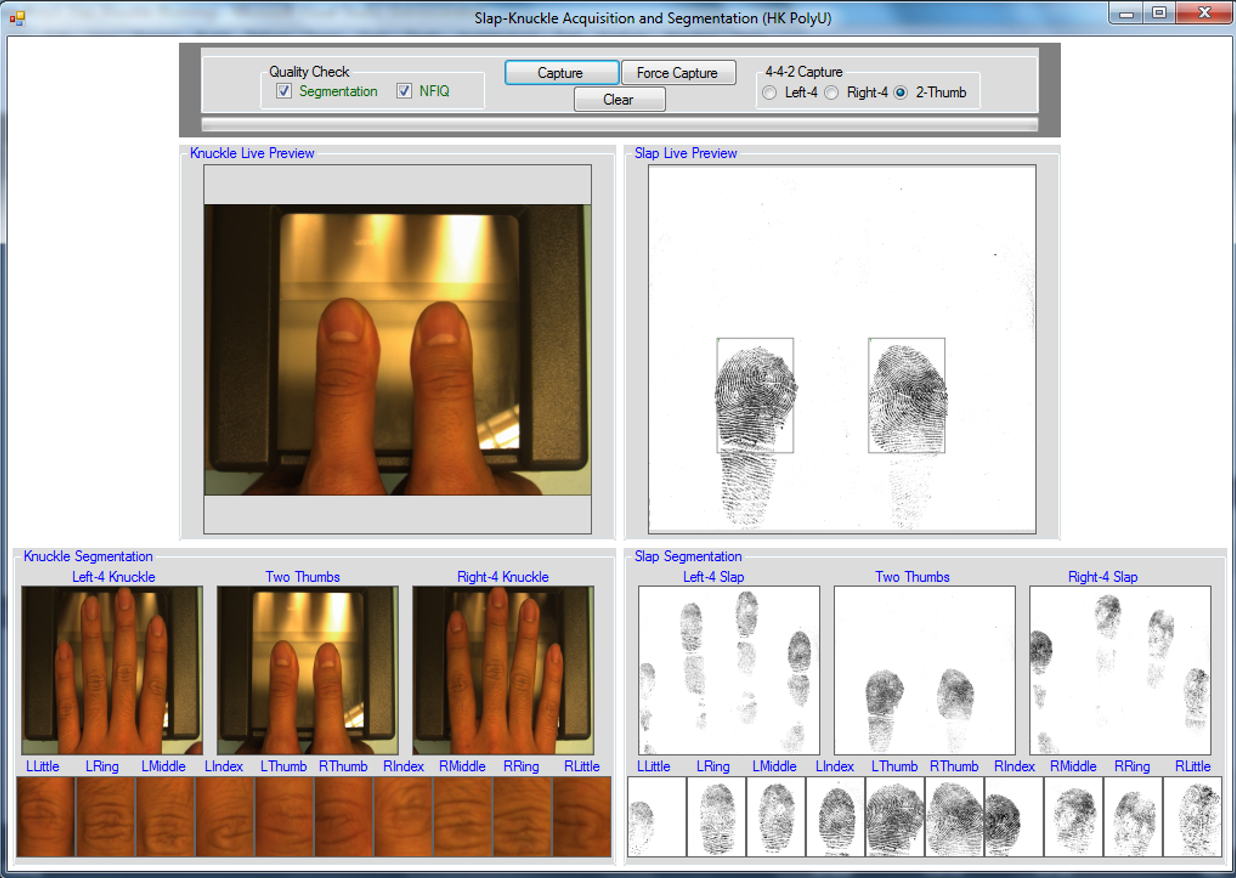
\includegraphics[width=4in]{Figures/system.png}%
    \label{system-a}}
    \hspace{0.1in}
    \subfloat[]{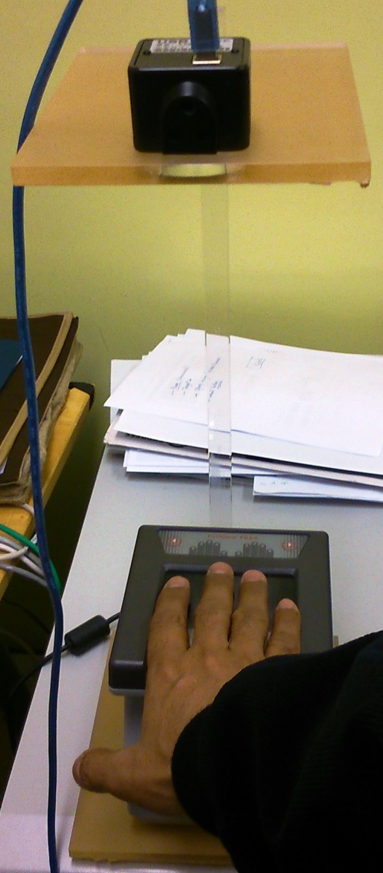
\includegraphics[width=1.250in]{Figures/system-sensor.png}%
    \label{system-sensor}}
    \caption{Online user authentication using slap-fingerprint and finger-knuckle images: (a) joint user interface developed for the 4-4-2 protocols (b) sensor placement for single shot imaging.}
    \label{system}
\end{figure*}

\subsection{Motivation and Our Work\label{motivation-contribution}}

The NIST report submitted to the US Congress \cite{2002SUMMARYON} underlines that about 2\% of the user population does not have usable fingerprints. NIST studies have also reported a false positive identification rate (FPIR) of ten-finger identification in the range of 1.5 to 3.5\% on a gallery size of about one million. Similar conclusions have also been reported in a large-scale proof-of-concept study undertaken by UIDAI \cite{uidai}. This study indicated that about 1.9\% of the subjects could not be reliably authenticated by only using their fingerprints. One of the critical challenges with large-scale deployed fingerprint authentication systems is also related to the acquisition of fingerprint images, and such sensing requires a fair degree of cooperation from the users. Therefore, it is not uncommon in the literature to report a failure to enroll (FTE) rate in the range of 1\% to 5\% for fingerprints. 

The drawback of currently popular fingerprint-only user identification can be complemented by incorporating finger knuckle information for user identification. Besides, there are several advantages of the new system. First, the data collection facility is easy to set with a low cost. Second, the data collection procedure is simple. Since the finger knuckle and fingerprint data can be collected simultaneously, no extra time is needed. Third, users will have almost the same user experience without any confusion. The key idea of this paper is to develop a finger-knuckle-assisted fingerprint identification system to significantly improve user identification accuracy without causing additional user inconvenience. To achieve this goal, firstly, the fingerprint and finger-knuckle data of each user must be acquired simultaneously and with a single imaging shot; secondly, both fingerprint and finger-knuckle must be accurately segmented and aligned; finally, a dynamic fusion strategy must be introduced to accommodate degradation in the fingerprint and finger-knuckle quality and significantly enhance user the identification capabilities.

The key contributions from this paper can be summarized as follows: 

\begin{itemize}
    \item This paper introduces a new biometric system, i.e. finger-knuckle-assisted fingerprint identification system, to address current limitations from widely deployed slap-fingerprint sensors at border crossings and national ID programs. This system simultaneously acquires fingerprint and finger-knuckle images with a single imaging shot, with no additional user inconvenience or degradation in traffic flow, and can serve as an add-on system for the existing or the deployed slap fingerprint systems. Our research introduces more effective finger knuckle segmentation capabilities from the finger dorsal images acquired under complex backgrounds, ambient illumination, and in the present multiple finger knuckles that are inherently observed in such simultaneously acquired images. We incorporate dynamic fusion capabilities to address the limitations resulting from degraded fingerprint or finger-knuckle images. Our experimental results presented in this paper validate the effectiveness of the proposed biometric system for its usage in a range of real-world applications. 
    \item We develop the first joint finger-knuckle and fingerprint database, which has been acquired from 120 different subjects, using 4-4-2 imaging protocols, and introduced in the public domain. To the best of our knowledge, there is no such joint database developed or available so far, and its availability in the public domain will help to advance further research and development efforts for the real-applications. 
    \item \textcolor{red}{We propose a new finger knuckle recognition framework, called \textit{RS-SSIM}, which can outperform the state-of-the-art finger knuckle method regardless based on non-deep learning or deep learning from the Fig. \ref{compare-fingerknuckle}. The new method can rotate and shift template generated from convolution neural network for getting more robust structural similarity index measure (SSIM) \cite{wang2004image}, although CNN and SSIM are rotational and translational variance.} 
\end{itemize}


The rest of this paper is organized as follows. Section \ref{fk-acquire} introduces a single-shot imaging-based framework for finger-knuckle-assisted slap fingerprint identification. This section also details the finger knuckle segmentation strategy developed to automatically segment finger knuckle images from the slap finger dorsal images acquired under complex and ambient imaging backgrounds. Section \ref{template-generation} introduces a dynamic scheme to consolidate finger knuckle and fingerprint match scores while Section \ref{experiment} presents the experimental results. Section \ref{discussion} presents a discussion and the key conclusions of this work are summarized in Section \ref{conclusion}.

\section{Finger Knuckle Acquisition and Segmentation}

We incorporated an FBI compliant slap-fingerprint scanner and a digital camera to simultaneously acquire finger-knuckle images. Such imaging setup, as shown in Figure 1, acquires finger knuckle images under ambient illumibation and background. Each of the subjects are imaged using 4-4-2 mode slap fingerprint acquisition [19] as for the case during their deployments at border crossings or enrollments during national ID programs. The acquisition of finger knuckle images is simultaneously, and corresponding to 4-4-2 to fingerprints images. Figure 2 illustrates sample finger dorsal images that are simultaneously acquired from the additional camera located above the slap-fingerprint sensor. These images also show automatically detected finger knuckle region contours for the feature extraction. The images in Figure 3 illustrate simultaneously acquired fingerprint images from a slap fingerprint sensor, corresponding to a user with knuckle images in Figure 3.

The block diagram for the finger-knuckle assisted slap fingerprint identification system is shown in Figure 4. Acquisition of finger-dorsal surface images is synchronized with the slap-fingerprint image acquisition and therefore the two images are acquired using a single imaging shot. The finger knuckle images are acquired under ambient illumination, which inherently present complex background resulting from the slap-fingerprint sensor surface. Therefore these images are firstly subjected to the preprocessing operations to normalize the illumination. The key task is to accurately localize, i.e., detect and segment, four (or two) finger knuckle regions from such simultaneously acquired images. Section 2.1.1 explains our approach to automatically segment desired finger-knuckle regions from the acquired images. Each   of   the   detected   knuckle   region   images  are  firstly normalized to ensure are  firstly normalized to ensure alignment among segmented knuckle regions from the successive images and the approach detailed in Section 2.1.2. Detected finger knuckle regions are subjected to the feature extraction steps, to generate respective templates. These templates are matched during the user authentication to generate the respective finger-knuckle match score. The segmentation of fingerprint images is relatively easier, or quite matured, and such segmentation algorithms are widely provided with commercial slap-fingerprint sensor. Each of the segmented fingerprint images are subjected to the feature extraction to generate respective fingerprint templates. These templates are matched with the corresponding fingerprint templates, stored in the registration database, to generate respective fingerprint match score during the user authentication. Two simultaneously generated match scores, from the fingerprint and respective finger-knuckle images, are subjected to a dynamic fusion algorithm (as detailed in Section 3) to generate a consolidated match score for the user authentication.  

\subsection{Finger Knuckle Segmentation from Single-Shot Images}
\subsubsection{FINGER KNUCKLE DETECTION FROM MULTIPLE FINGERS}
Each of the simultaneously acquired, i.e. single-shot images during 4-4-2 imaging, knuckle images present multiple finger dorsal surfaces. Finger knuckle detectors introduced in the literature [7] designed for images under uniform background and/or for the single finger dorsal surfaces. However the slap-fingerprint finger dorsal surface images present multiple fingers, which may be in full contact (see sample in Figure 2f) with each other and acquired under complex background with ambient illumination. Therefore finger-knuckle detectors employed in earlier research [6] cannot be employed to address our detection task. We therefore developed a specialized mask R-CNN [15] based finger-knuckle detector for our system. The mask R-CNN [15] has shown its superior performance in object detection and segmentation tasks, for example we can observe impressive results for the COCO object detection and segmentation competition. Therefore, we developed a finger knuckle detector using the mask R-CNN framework as shown in Figure 5. Finger Knuckle images are fed into a standard CNN network (we use ResNet [30] here) and a Feature Pyramid Network (FPN) [11] to build multi-scale RoI features. From RoI features, Region Proposal Network (RPN) generates finger knuckle region proposals, which will be processed by RoIAlign to further improve finger knuckle localization. Mask R-CNN generates three outputs: finger knuckle class label, finger knuckle bounding box, and finger knuckle segmentation mask. The finger knuckle detector training samples were collected from a separate subject whose images are not included in the finger-knuckle and fingerprint database. Since knuckle detection is not a complex task, we used ResNet-50 FPN as the backbone instead of ResNet-101 FPN. We used data augmentation [27], such as random rescaling, horizontal flipping and color jittering, to augment the training data. We also used contrast enhancement, during the preprocessing stage, to normalize the acquired images that are acquired under varying illumination. 

The mask R-CNN generates several bounding boxes that may or may not contain finger knuckle and therefore. The reason is that the bounding box may indicate minor finger knuckle, or region that may look similar to the finger knuckle. In this work we only consider the major finger knuckle as the region of interest, i.e., in rest of this paper the term finger knuckle refers to the major finger knuckle. The bounding boxes that are generated by Mask R-CNN indicate possible locations of finger knuckles, and bounding boxes with higher confidence scores most likely the regions with correct localizations of the finger knuckle regions. Therefore, to identify the correct bounding box with the finger knuckle regions, we firstly assume that the bounding box with high confidence scores are more likely to indicate the finger knuckle. Secondly, the bounding box with high confidence score may still indicate incorrect location of finger knuckle. Therefore, we propose to incorporate the domain knowledge, i.e. relative geometric locations of the finger knuckle regions, to improve the finger knuckle detection capability. For the human finger knuckles, four finger knuckles on the acquired images are expected to be in a relative sequence along the horizontal or x-axis. Along the vertical or y-axis, middle finger knuckle and ring finger knuckle are expected to be higher than the index finger knuckle and ring finger knuckle. Finally, along the vertical axis, all four knuckles are not expected to be far away from each other.

We designed an algorithm to automatically determine the four bounding boxes or the regions of our interest. This algorithm can be summarized as follows: firstly, we choose four bounding boxes with the top four highest confidence score and check if they are compliant with their expected geometrical distribution. In absence of such compliance, we automatically remove the incorrect bounding box, from the rest or the shortlisted bounding boxes, choose the one with the highest confidence score. As shown in Algorithm 1, we repeat this process until all the bounding boxes, or the chosen regions, are compliant with their expected geometrical distribution.

The Algorithm 1 can be briefly explained as follows. Step 1 firstly generates the set of all bounding boxes  (Figure 6) that may include finger knuckle like patterns. Each bounding box  is represented by top-left coordinate , bottom-right coordinate , and a corresponding confidence score  ranging from 0 to 1. Step 2 to Step 6 selects bounding boxes with highest confidence scores and sort them along horizontal axis. In step 8, for simplicity reason, the top-left coordinate of each bounding box is represented by , because only top-left coordinate is required for the later use. Also, for the reasons of simplicity, the top-left coordinate is used to identify the location of each of the bounding boxes. The coordinate of each bounding box is normalized with respect to the width and height of the image. For normalization, given the height and the width of the image, the vertical and horizontal coordinate of the bounding box is normalized by the height or the width respectively. The variables that are computed from step 8 are used to control the geometrical distribution of the four bounding boxes so that they are compliant with the expected geometrical distribution of four knuckles. The variable  in equation (2) is computed to ensure that along the vertical axis two locations, i.e. the bounding box on the top and at the bottom, are not far away from the other bounding boxes. The variables , ,  and  in equation (3)-(4) are similarly used to check the two knuckle locations in the middle (for slap finger image, the two knuckles correspond to middle knuckle and ring knuckle) so that these two knuckles are closer to each other. These are guaranteed by constraints in (1) and (2). Similarly, the constraints in (3)-(6) are used to check the validity of knuckle locations on both sides. The constraints in (3) and (5) ensure that the appearing locations at the bounding box is valid for the left-most knuckle (the left-most knuckle correspond to little knuckle of left hand and index knuckle of right hand). Similarly, the constraints in (4) and (6) are incorporated to ensure that the bounding box location is valid for the right-most knuckle (the right-most knuckle correspond to index knuckle of left hand and little knuckle of the right hand). The parameter  and  in equation (6) are used to discard the possibility that the two bounding boxes are located or detected on the one/same finger. The hyperparameters in Step 9 are empirically selected and for all our experiments in this paper we fixed , , , , and .

\subsubsection{Finger knuckle alignment and normalization}

As can be seen from a sample slap-fingerprint dorsal image in Figure 2 that the presented fingers from the users may not be strictly upright, and the extent of such finger knuckle orientation can vary for different fingers even in the same image. Therefore, the orientation of finger-knuckle regions also varies for each of the fingers. In absence of any orientation normalization, the match accuracy between different knuckle images can significantly degrade. We therefore automatically estimate the orientation for each of the fingers present in the acquired image and incorporate alignment in the segmented or normalized finger knuckle images.

The orientation of finger knuckle region is inherently linked with the orientation of the fingers presented on the slap-fingerprint sensor. Therefore, a trained Mask R-CNN is used to detect the fingers. Based on the segmented finger area from this finger detector, a rotated rectangular bounding box with minimum area is fitted. The orientation of the largest side of this rectangle indicates the orientation of the respective finger. Figure 8 illustrates a sample image and such estimated orientation for each of the fingers in this image. The orientation of each of the fingers is used to automatically segment the aligned or normalized finger knuckle images for the feature extraction. Figure 9 illustrates the effectiveness of   such   orientation   alignment   where   the   segmented images without alignment and respective images after alignment are shown from a sample image in our database. Table 1 presents a summary of estimated orientation for each of the fingers for the images in our database. It can be observed that the orientation of each finger knuckle region varies, and the average orientations of the same finger knuckle, from the left hand and the right hand, are quite close to each other.


\section{Template Generation and Matching}

\subsection{Finger Knuckle Template Generation}

Each of the segmented and normalized finger-knuckle images are subjected to the feature extraction to generate respective templates for the matching. There are a range of spatial domain [5]-[6], [8]-[9], [12]-[13] and spectral domain [24]-[25] methods investigated in the literature to match finger knuckle patterns. Among these methods spatial-domain methods are quite attractive as they are computationally simpler and have shown to offer state of the art results.  We employed the local feature descriptor based approach introduced in [12]-[13] to generate finger knuckle templates as this approach is computationally attractive, accurate and generates smallest finger-knuckle templates (one-bit-per-pixel) that can be more conveniently stored along with the fingerprint-templates for the real applications. 

\subsection{Fingerprint Template Generation}

Among a range of methods introduced in the literature [3] to match fingerprint images, minutiae-based methods are widely employed and therefore preferred. We considered a range of popular methods and implementations available in the references to generate fingerprint templates. Among various fingerprint matchers employed in the literature, NBIS (NIST Biometric Image Software) [17] and minutiae cylinder code (MCC) [18] are quite popular. We also considered a commercial off-the-shelf (COTS) matcher [16] which has shown quite accurate results in many references. Simultaneously acquired fingerprint images from the slap-fingerprint sensors are automatically segmented and employed to generate fingerprint templates. These templates are used to generate respective match scores that are consolidated for the user authentication. 

\subsection{Dynamic Score Consolidation}

The match scores generated from two independent pieces of evidences are consolidated to achieve a more reliable decision score for the user authentication. Biometrics literature [3] provides extensive investigation on a range of methods to consolidate decisions from two pieces of evidences or features. Such consolidation from can be achieved at feature level, score level, or at the decision level. The score level combination is most widely used in the literature and is widely adapted [31] in a range of biometrics system, largely due to its simplicity and the performance. The objective of our system is to serve as an add-on system on the top of existing or deployed slap-fingerprint system where the match scores are inherently available from the respective minutiae templates. Therefore, score level combination was preferred and adapted for the score consolidation in our system. 

Real biometric systems during their deployments are often presented with missing or degraded quality of biometric samples and therefore the score-level consolidation scheme should be adaptive to such inputs. Therefore, we developed a dynamic scheme to consolidate match scores from two simultaneously generated match scores from the fingerprint and the finger-knuckle. Let the match score from fingerprint be represented by  and the match score from the finger knuckle be represented by . The confidence or the quality of input biometric image sample, as shown in Figure 1, can be denoted as  and  respectively for the finger knuckle and fingerprint. The consolidated match score s is generated as shown in Algorithm 2. The weight w ( )  represents weight and is fixed empirically for all the experimental results in this paper. This scheme ensures that in case of missing or low quality biometric images, the importance is automatically granted for the other biometric modality.  
\section{Experiments and Results}

\subsection{Database and Protocols}

There is no public database on the simultaneously acquired finger-knuckle and fingerprint images from any slap-fingerprint sensor and this is the first system for the real applications in the best of our knowledge. Therefore, we developed an imaging setup to acquire the required database using an FBI compliant slap fingerprint sensor. We incorporated a commercial slap-fingerprint sensor [21] that also provides necessary drivers and SDK for the real applications. A 5M low-cost digital camera [29] was mounted on the top of slap fingerprint sensor and integrated to simultaneously acquire both biometric under single shot imaging. In order to acquire realistic finger-knuckle images for potential add-on solution with existing slap-fingerprint sensor deployments, so additional illumination was incorporated. Therefore, all the images were acquired under ambient illumination, in both indoor and outdoor environment.

The majority of the images in this database were acquired in India and none of the volunteers were paid for their contributions. All the volunteers aged between 11-62 and a large number of primary school students from a village in India contributed their images for this database. Each of the volunteers provided both right- and left-hand images in 4-4-2 protocol. We acquired 5 image samples from each of the subjects with each image sample acquired in 4-4-2 mode. Therefore, each subject provided a total of 30 images which included multiple fingerprint and finger knuckle images. A total of 120 subjects contributed to this database that included images from Indian, Chinese and European subjects. In order to advance further research and development efforts, the entire database acquired during this research is made publicly available via [22]. Segmented images from each of the finger knuckle and fingerprints were used to generate respective templates as discussed in Section 3 and employed for the matching. We employed more challenging matching protocol to ensure more reliable estimation on the performance from the two biometric images. Therefore, each of the fingers generated 1200 (120 ×10) genuine and 357000 (120×5×5×119) impostor match scores, for each of the fingerprint and finger knuckle images, and were used to ascertain the performance.  
\subsection{Performance from finger knuckle images\label{fk-performance}}

\begin{figure}[ht]
    \centering
    \subfloat[]{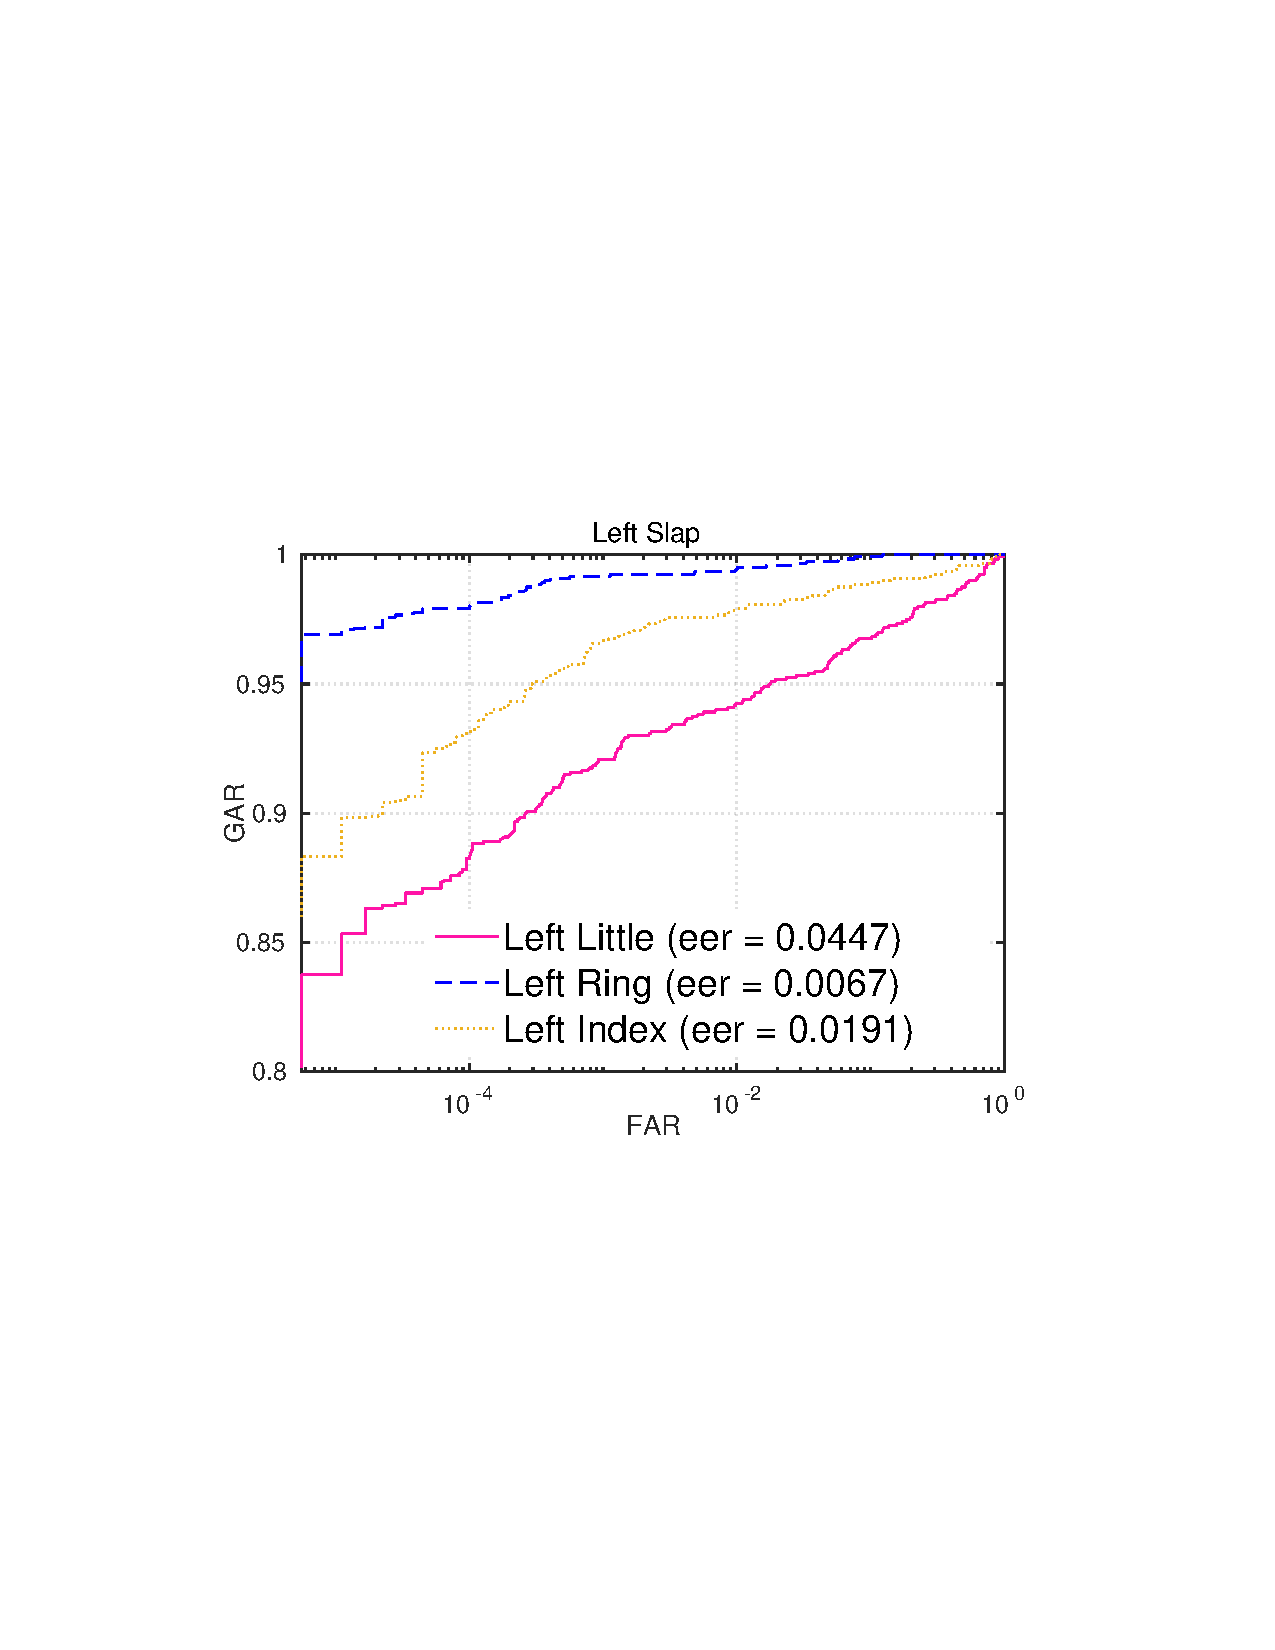
\includegraphics[width=1.7in]{Figures/finger-knuckle/left-roc.pdf}
    \label{}}
    \subfloat[]{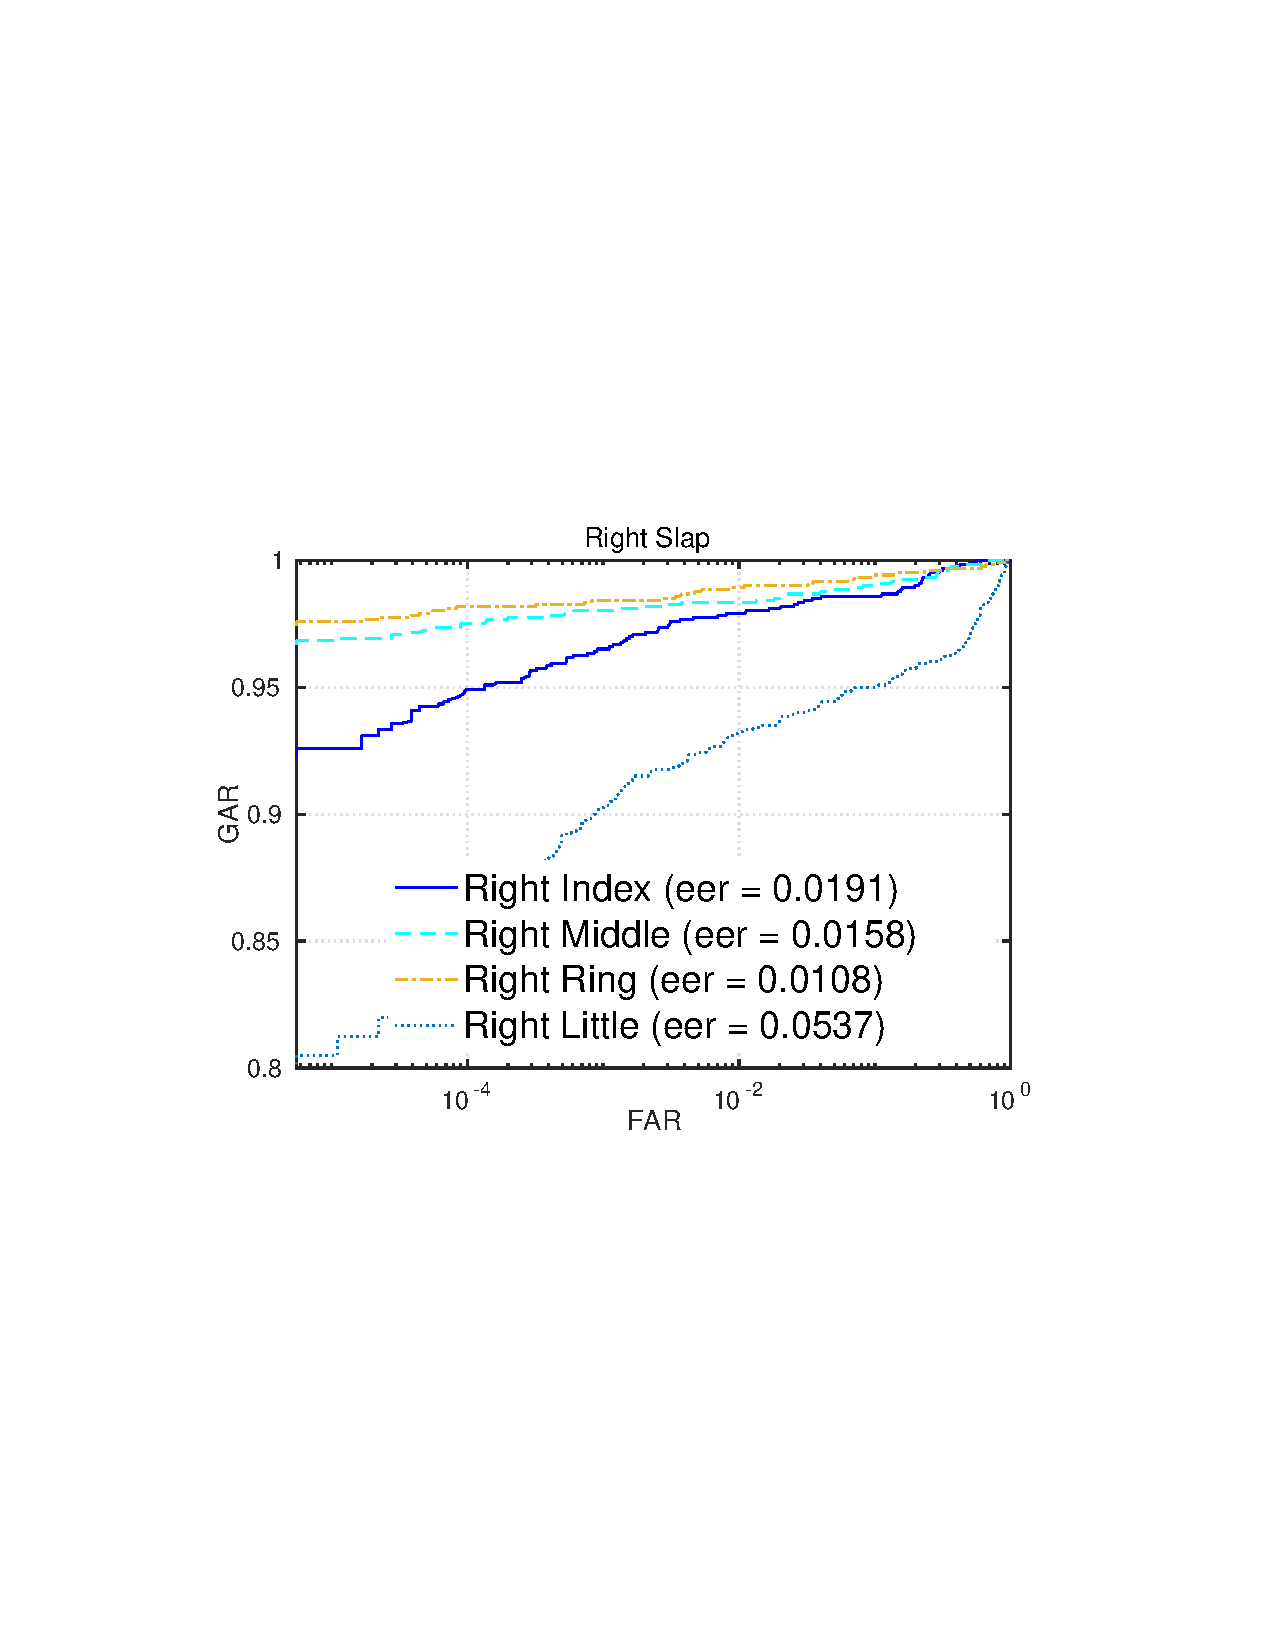
\includegraphics[width=1.75in]{Figures/finger-knuckle/right-roc.pdf}
    \label{}}

    \subfloat[]{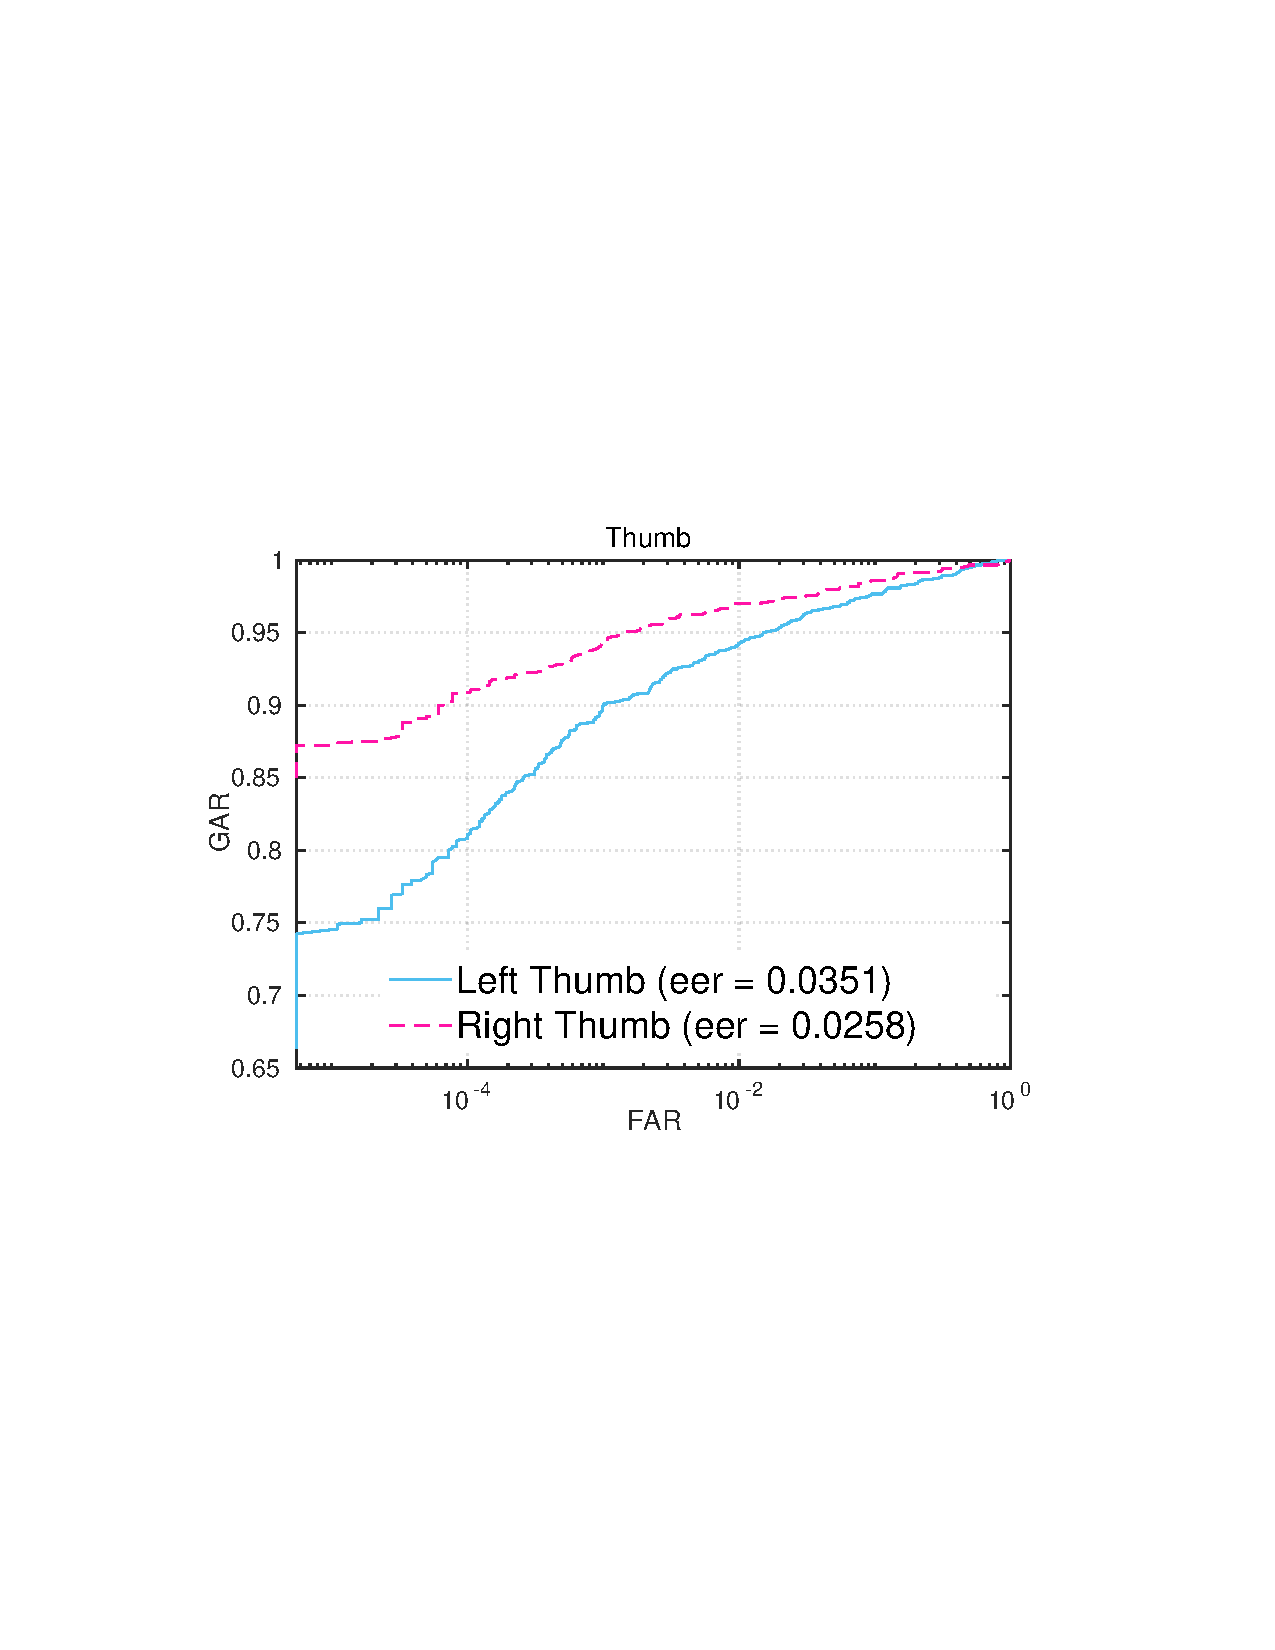
\includegraphics[width=1.8in]{Figures/finger-knuckle/thumb-roc.pdf}
    \label{}}
    \caption{Performance from the simultaneously acquired finger knuckle images from (a) left hand, (b) right hand, and (c) thumbs under 4-4-2 imaging protocols.}
    \label{fingerknuckle-performance}
\end{figure}

Each of the simultaneously acquired and segmented finger knuckle images were first evaluated for their individual performance. Fig. \ref{fingerknuckle-performance} illustrates receiver operating characteristics (ROC) for the finger knuckle images acquired from each of ten different fingers.  These results indicate that the ring finger knuckle, from both the hands, offers superior performance followed by the performance from the middle finger, and then index finger. The performance from the knuckle from thumbs and the little finger is observed to be relatively poor. This can be largely attributed to the high agility with the thumb and the little fingers which often results in degradation in the quality of segmented images. Figure 9 also illustrates the equal error rate (EER) values for the respective finger knuckle images. 

\textcolor{red}{Our method for finger knuckle recognition.}


\subsection{Performance from Fingerprint images\label{fp-performance}}

The performance from the fingerprint images acquired from each of the fingers in shown in Fig. \ref{fingerprint-performance}. A commercial fingerprint matcher is used for the fingerprint matching as it offered the best performance (more details in Section \ref{discussion}) among the three fingerprint matchers considered in this work. It can be observed from the ROC curves in these images that, unlike for respective finger-knuckle, the fingerprint images from the thumbs (thumbprints) offer the best performance. This is followed by the performance from the middle fingers. The thumbs are expected to generate superior performance and this can be attributed to the relative convenience during such imaging as the users find it easy to firmly press thumbs during the 4-4-2 fingerprint imaging. 

\begin{figure}[ht]
    \centering
    \subfloat[]{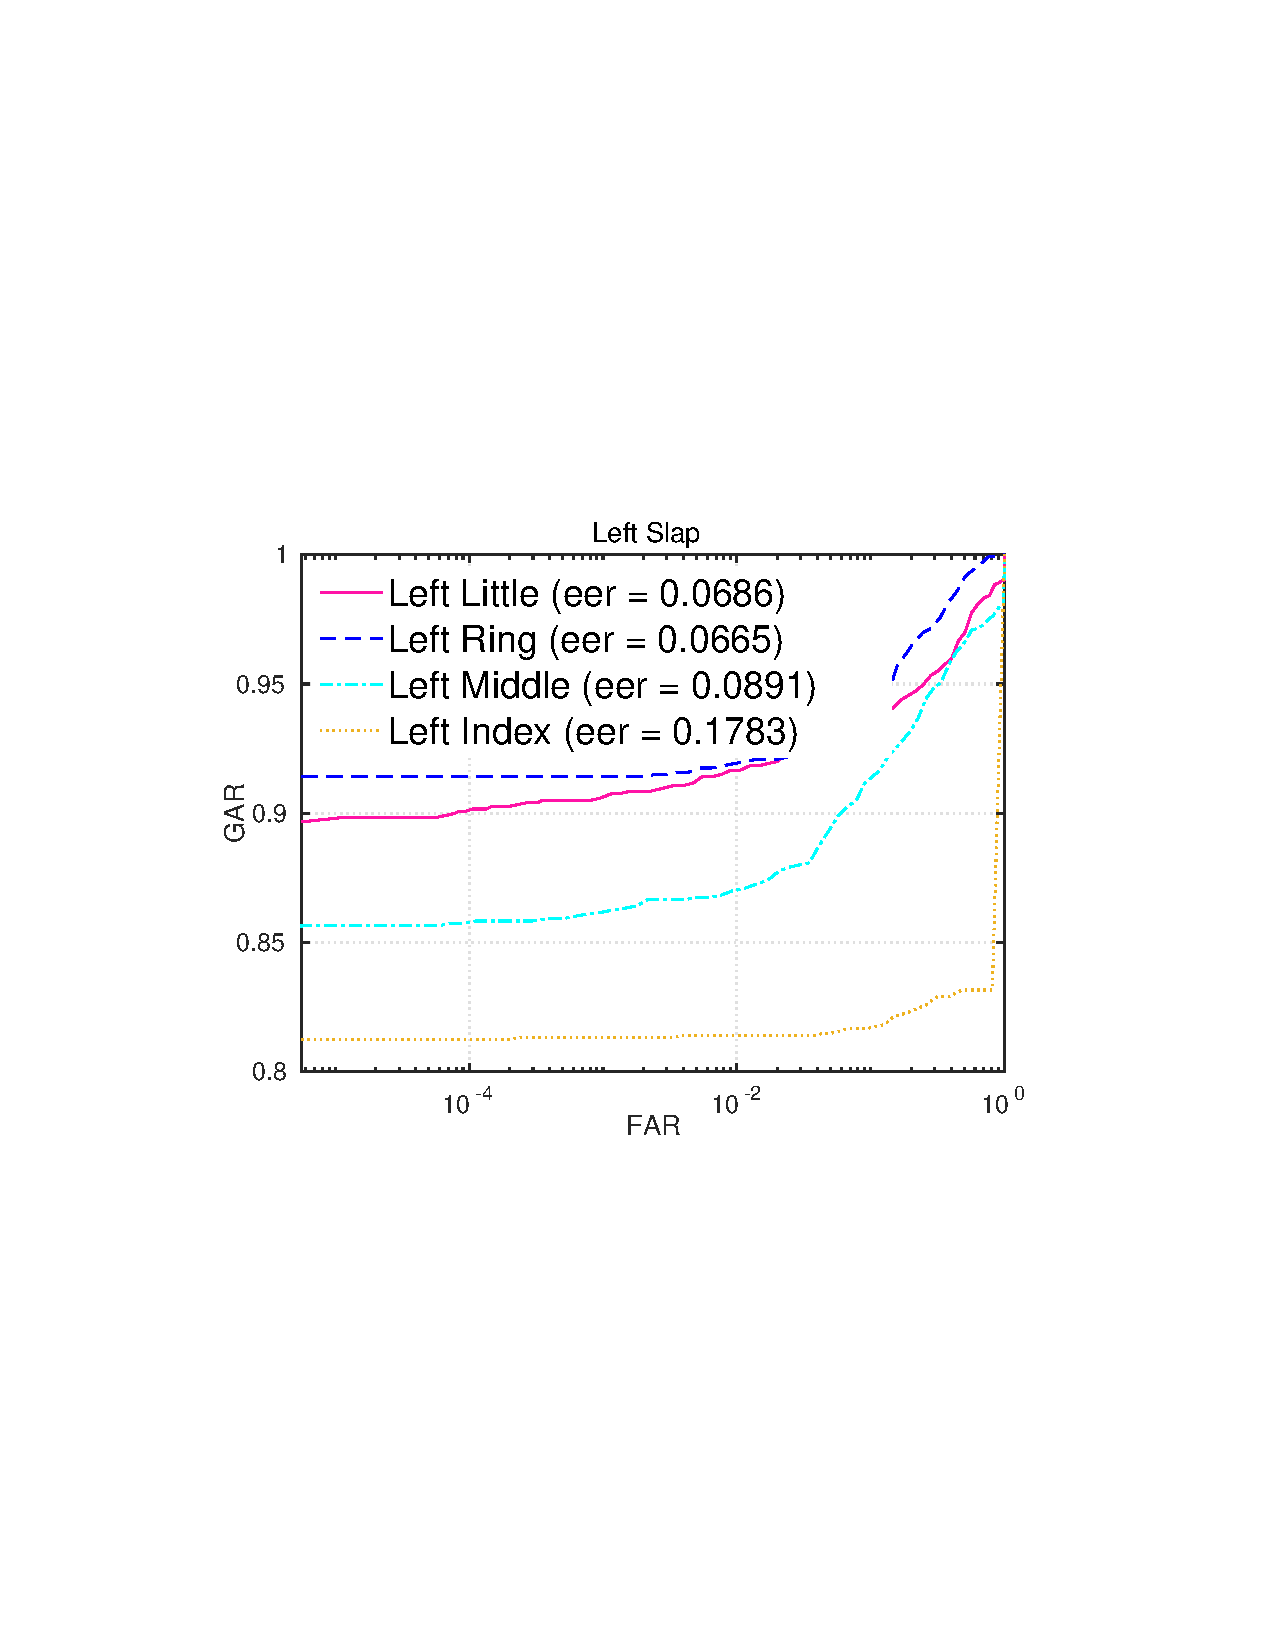
\includegraphics[width=1.7in]{Figures/fingerprint/left-roc.pdf}
    \label{}}
    \subfloat[]{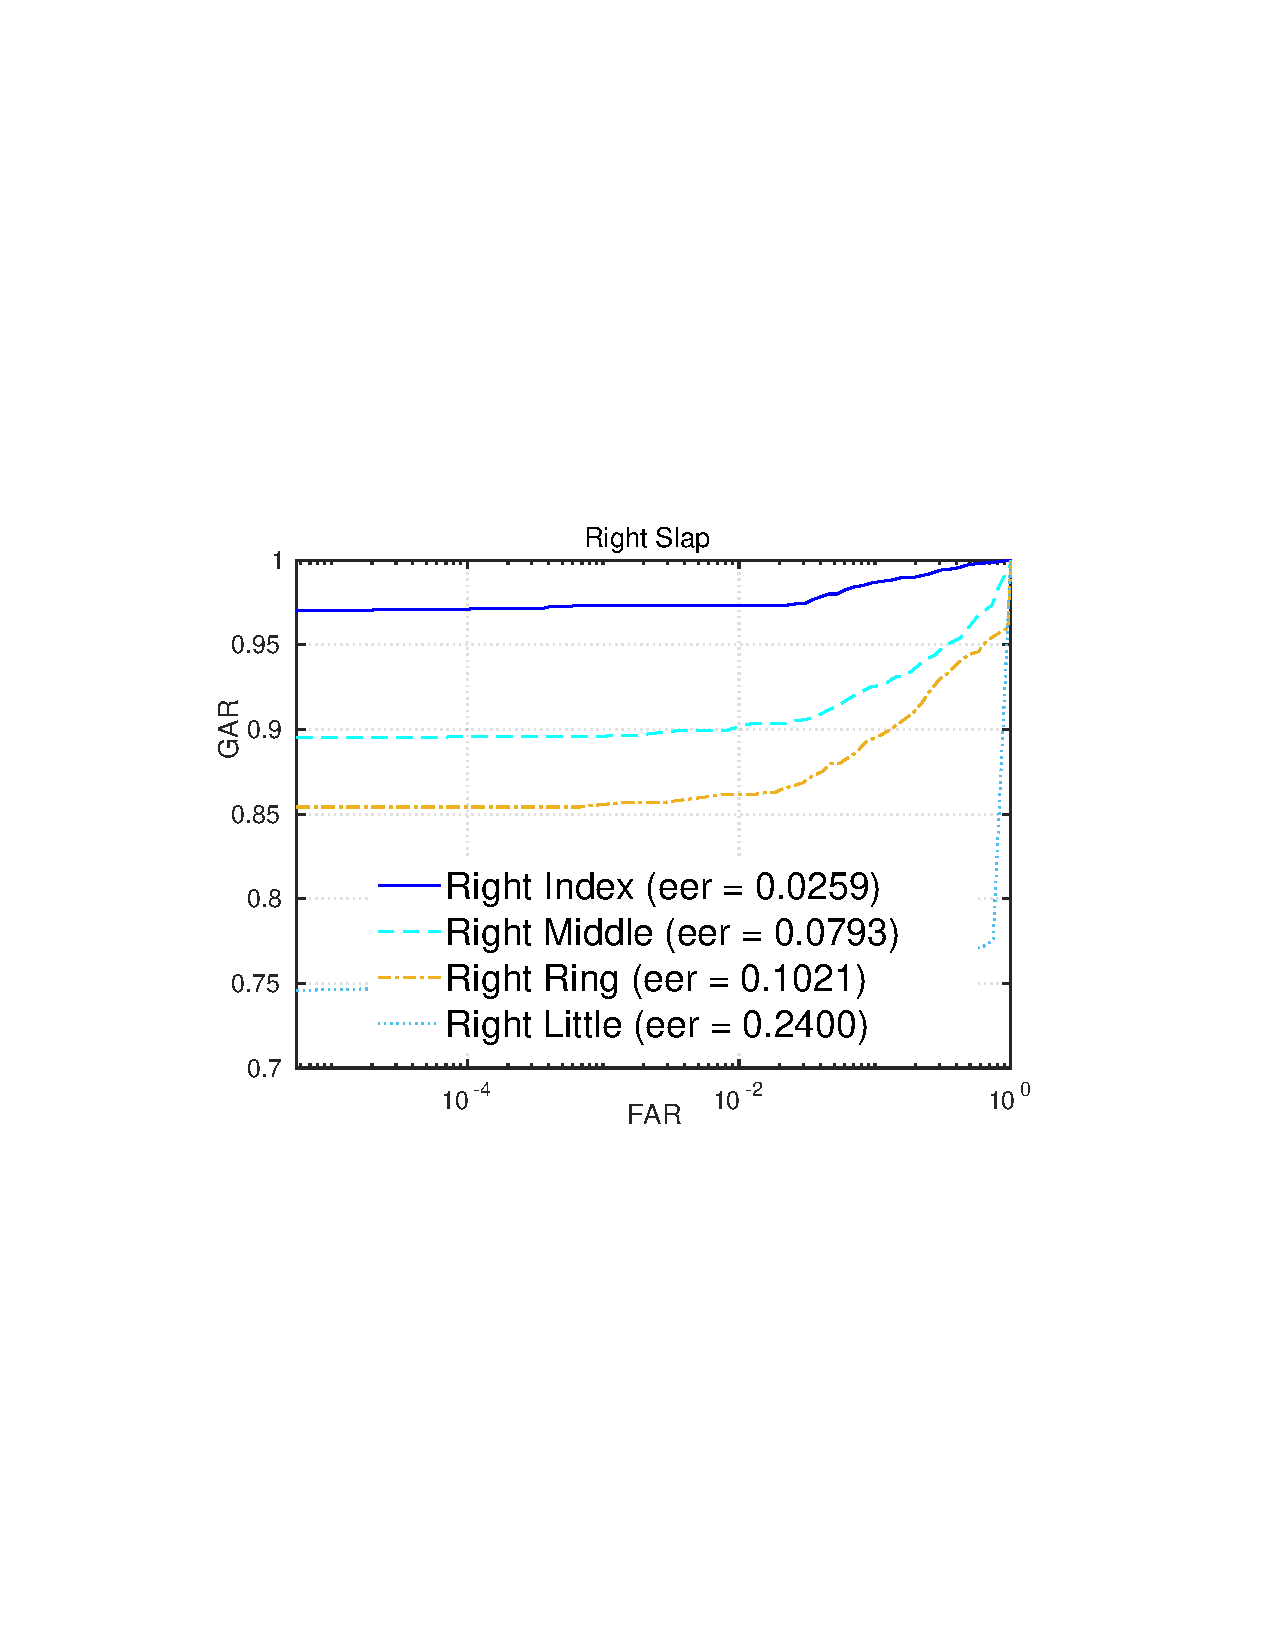
\includegraphics[width=1.75in]{Figures/fingerprint/right-roc.pdf}
    \label{}}

    \subfloat[]{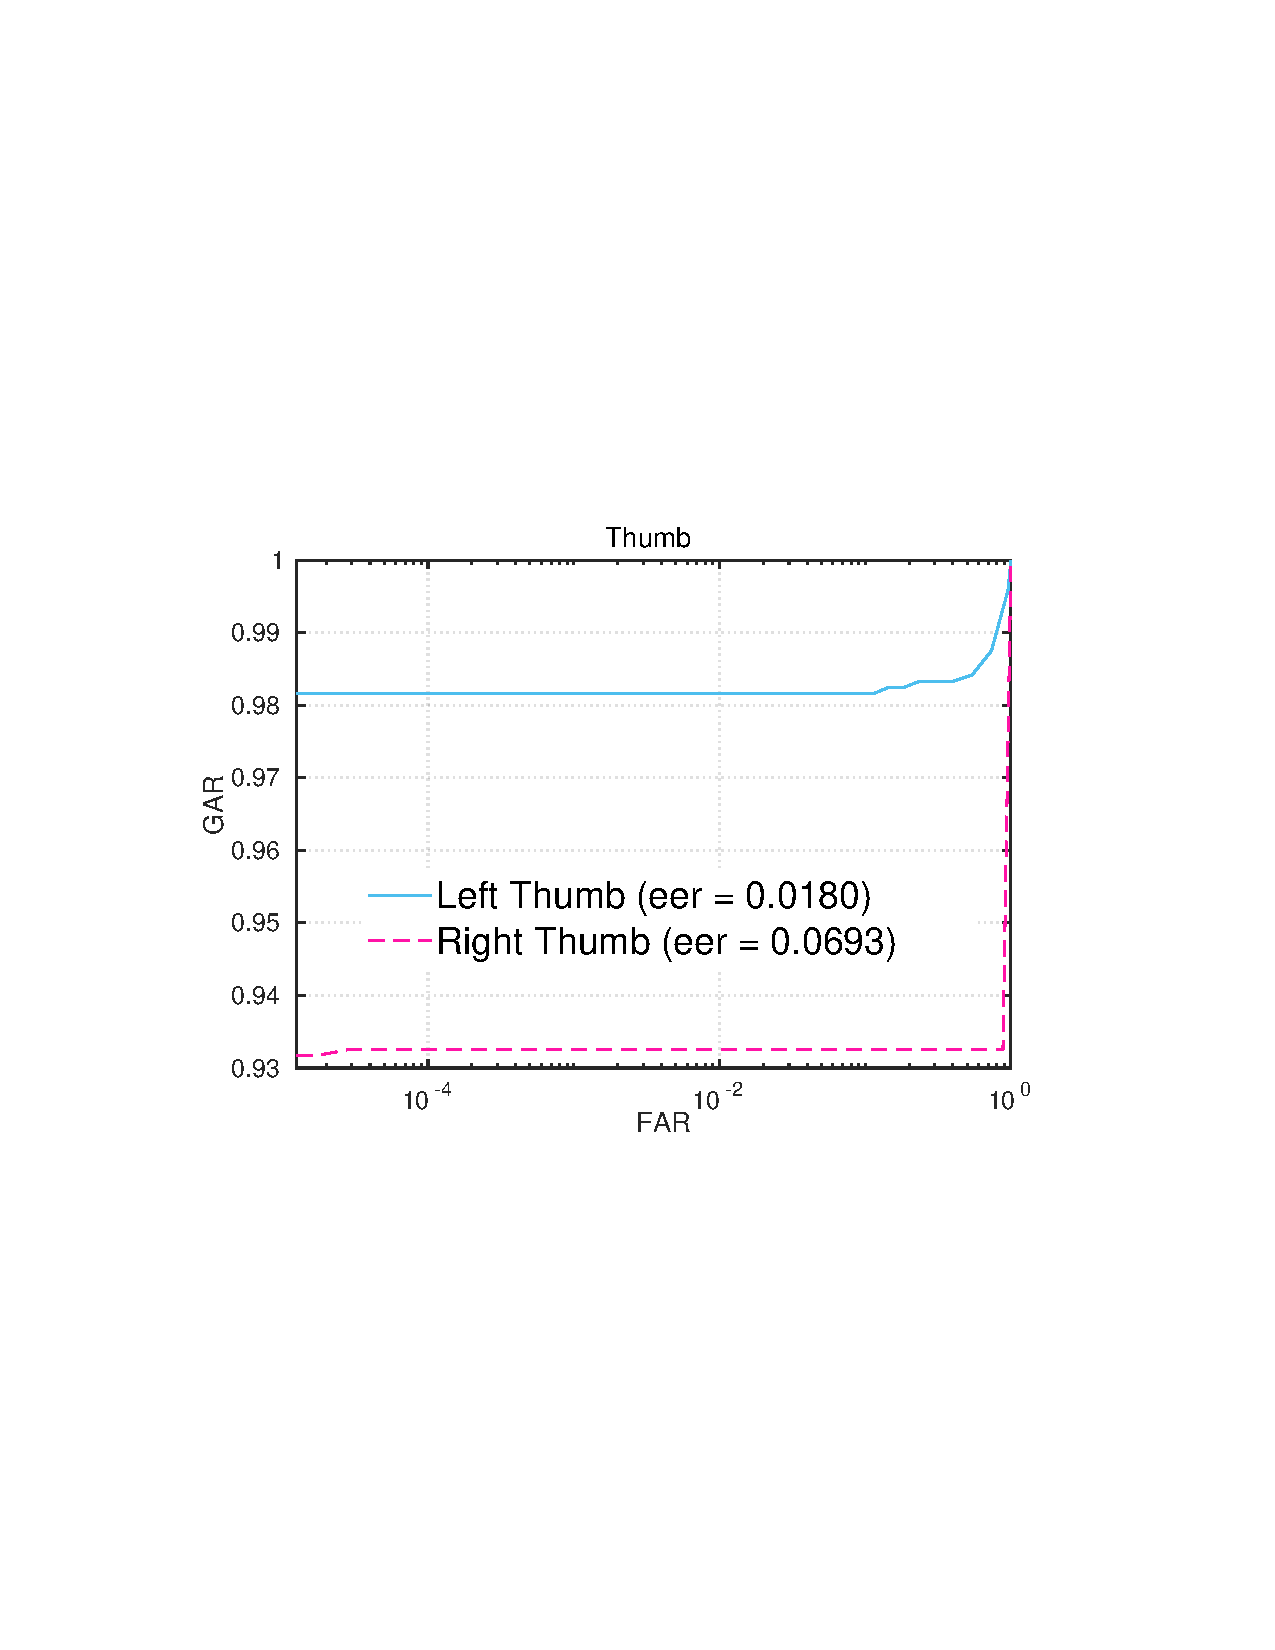
\includegraphics[width=1.8in]{Figures/fingerprint/thumb-roc.pdf}
    \label{}}
    \caption{Performance from the fingerprint images acquired using a slap-fingerprint sensor for (a) left hand, (b) right hand, and (c) thumbs under 4-4-2 imaging protocols.}
    \label{fingerprint-performance}
\end{figure}
\subsection{Joint Performance from Fingerprint and Finger Knuckle Images\label{joint-performance}}

\begin{figure*}
    \centering
    \subfloat[]{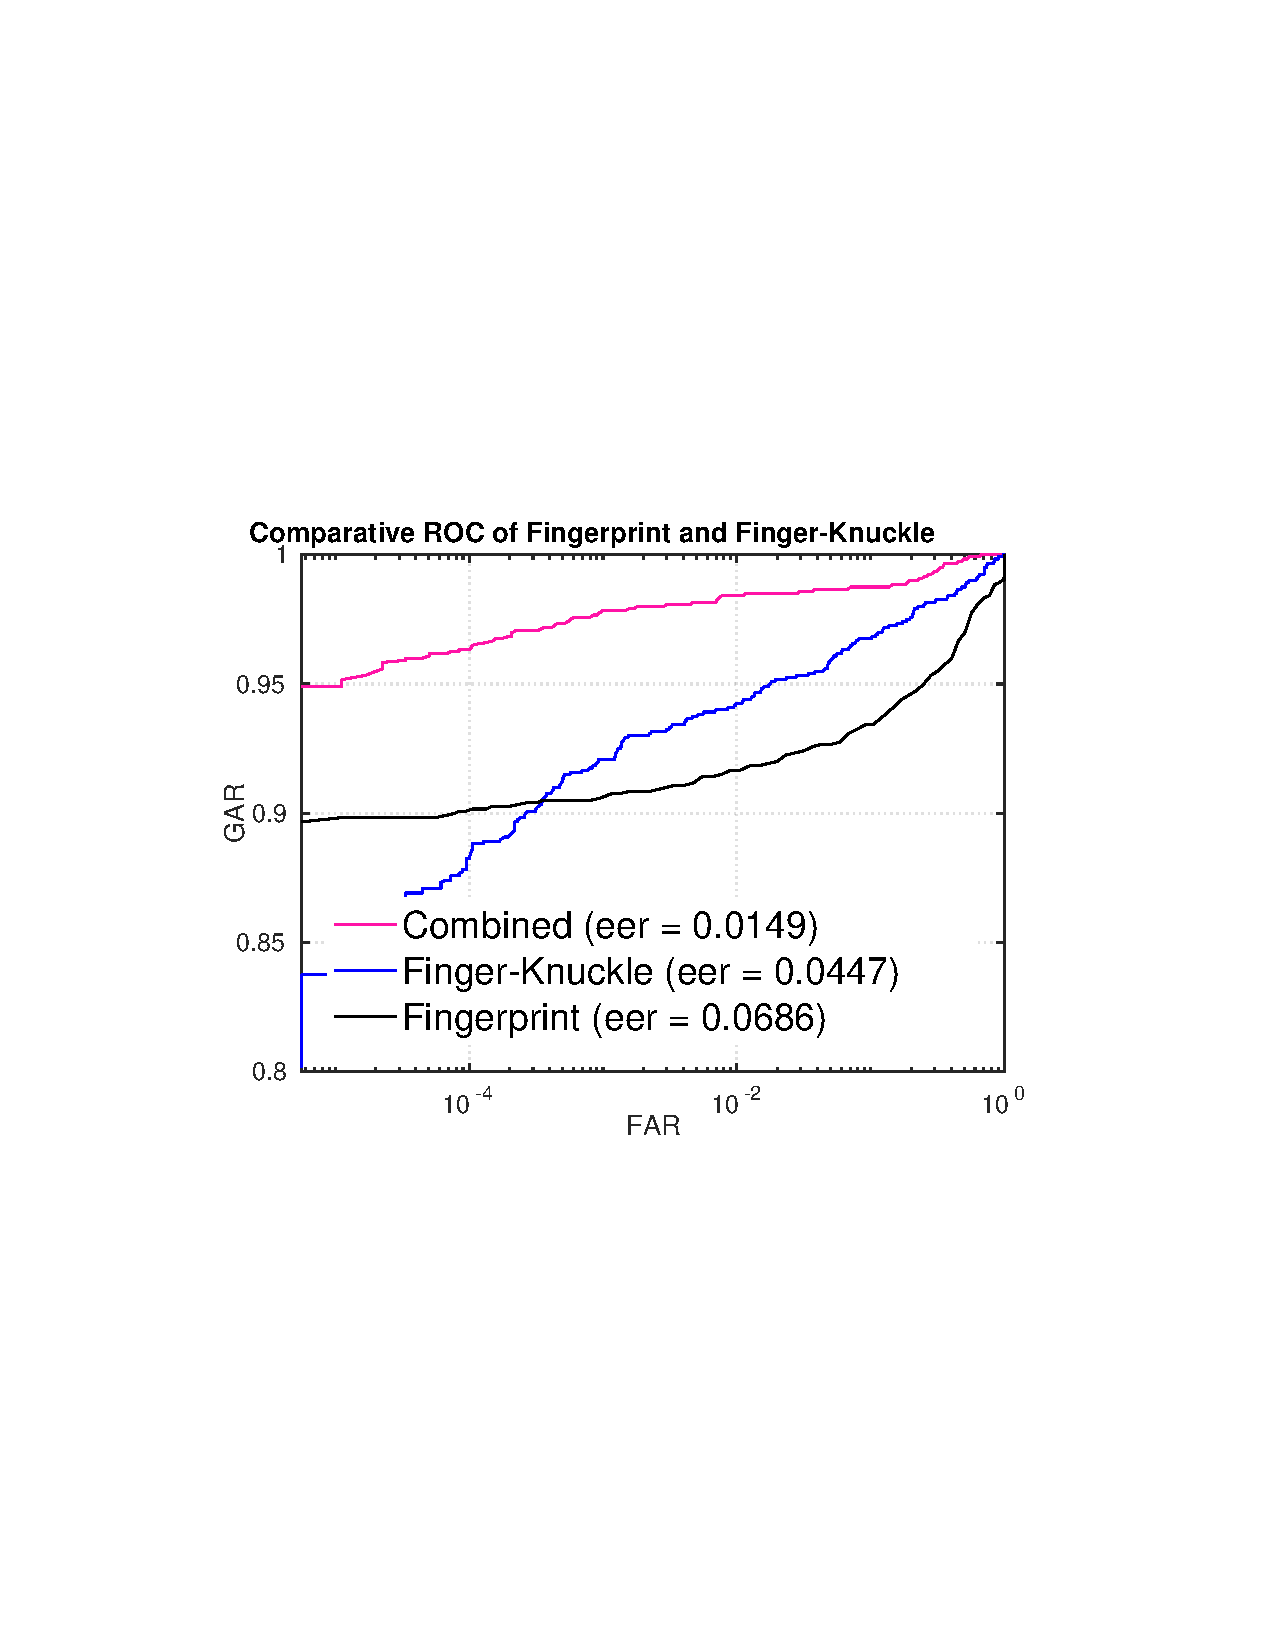
\includegraphics[width=2in]{Figures/dynamic/01.pdf}
    \label{}}
    \subfloat[]{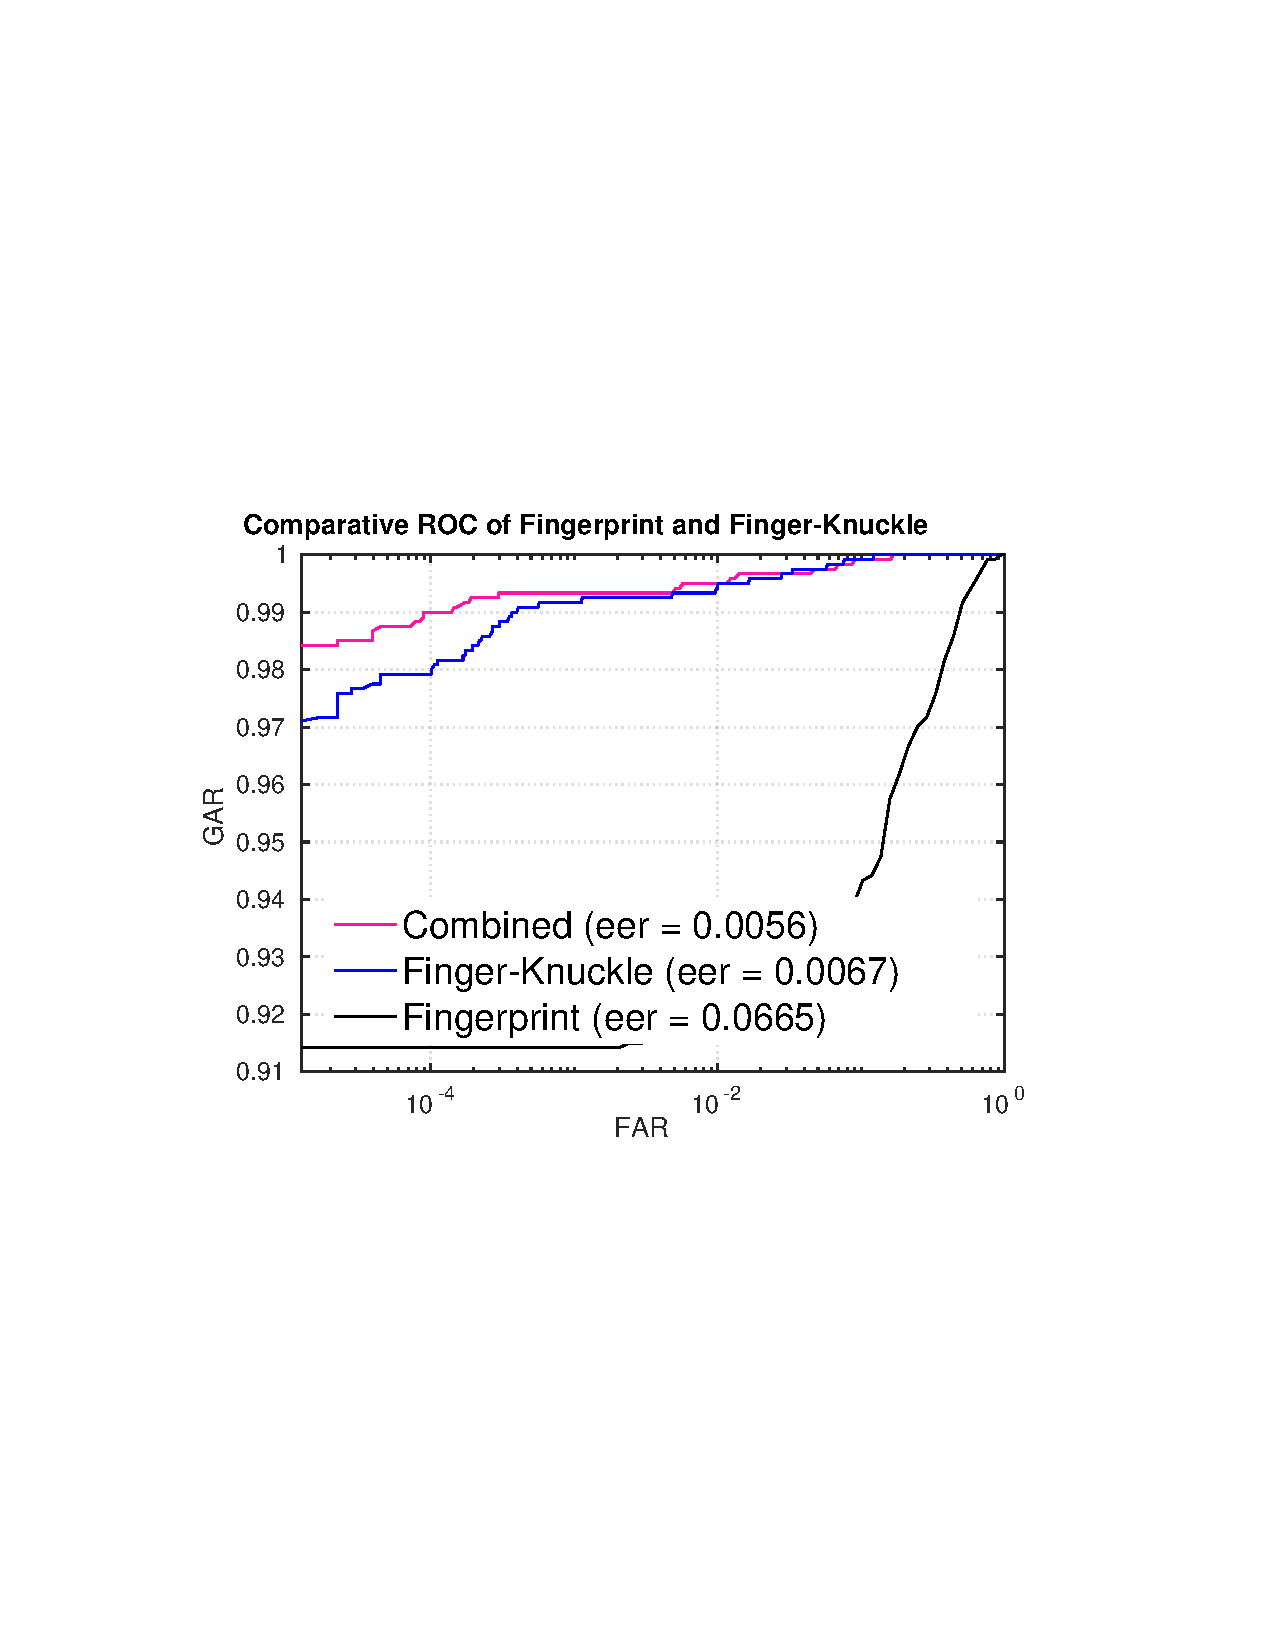
\includegraphics[width=2in]{Figures/dynamic/02.pdf}
    \label{}}
    \subfloat[]{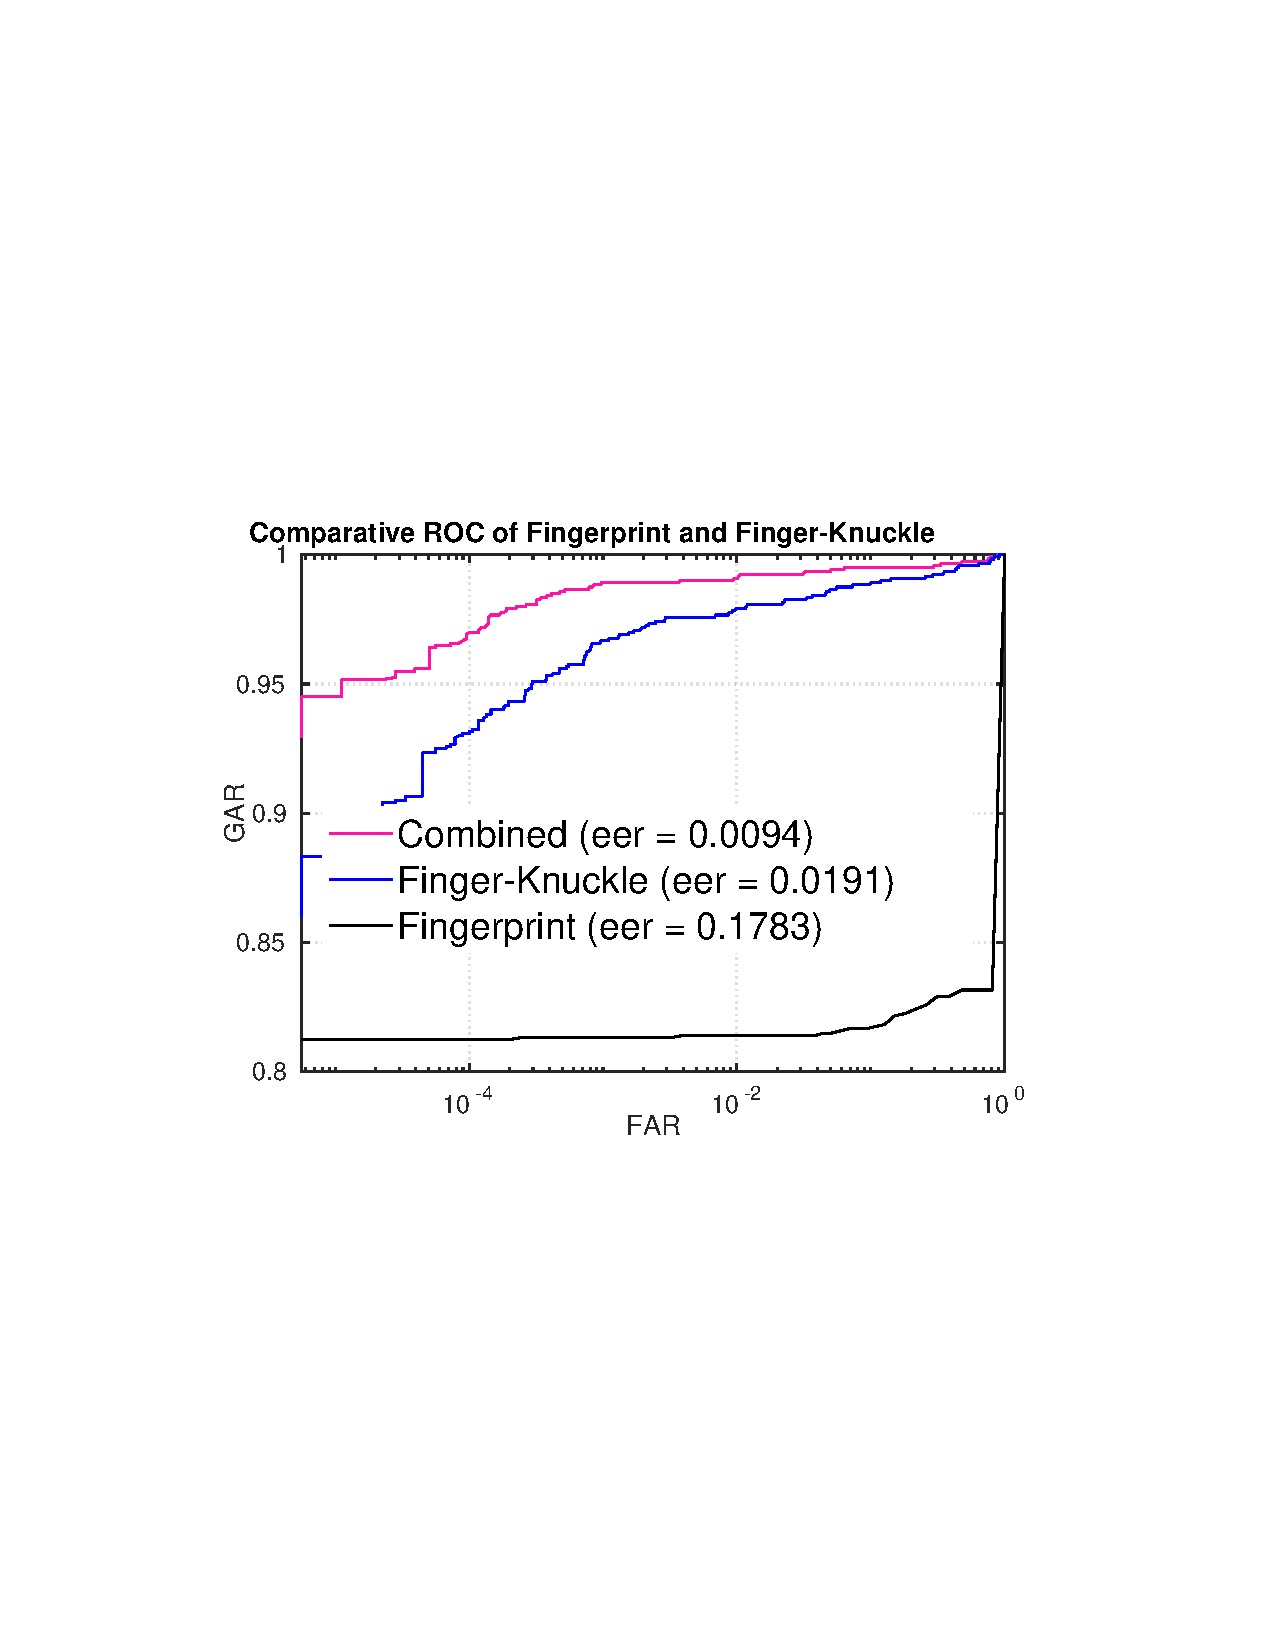
\includegraphics[width=2in]{Figures/dynamic/04.pdf}
    \label{}}

    \subfloat[]{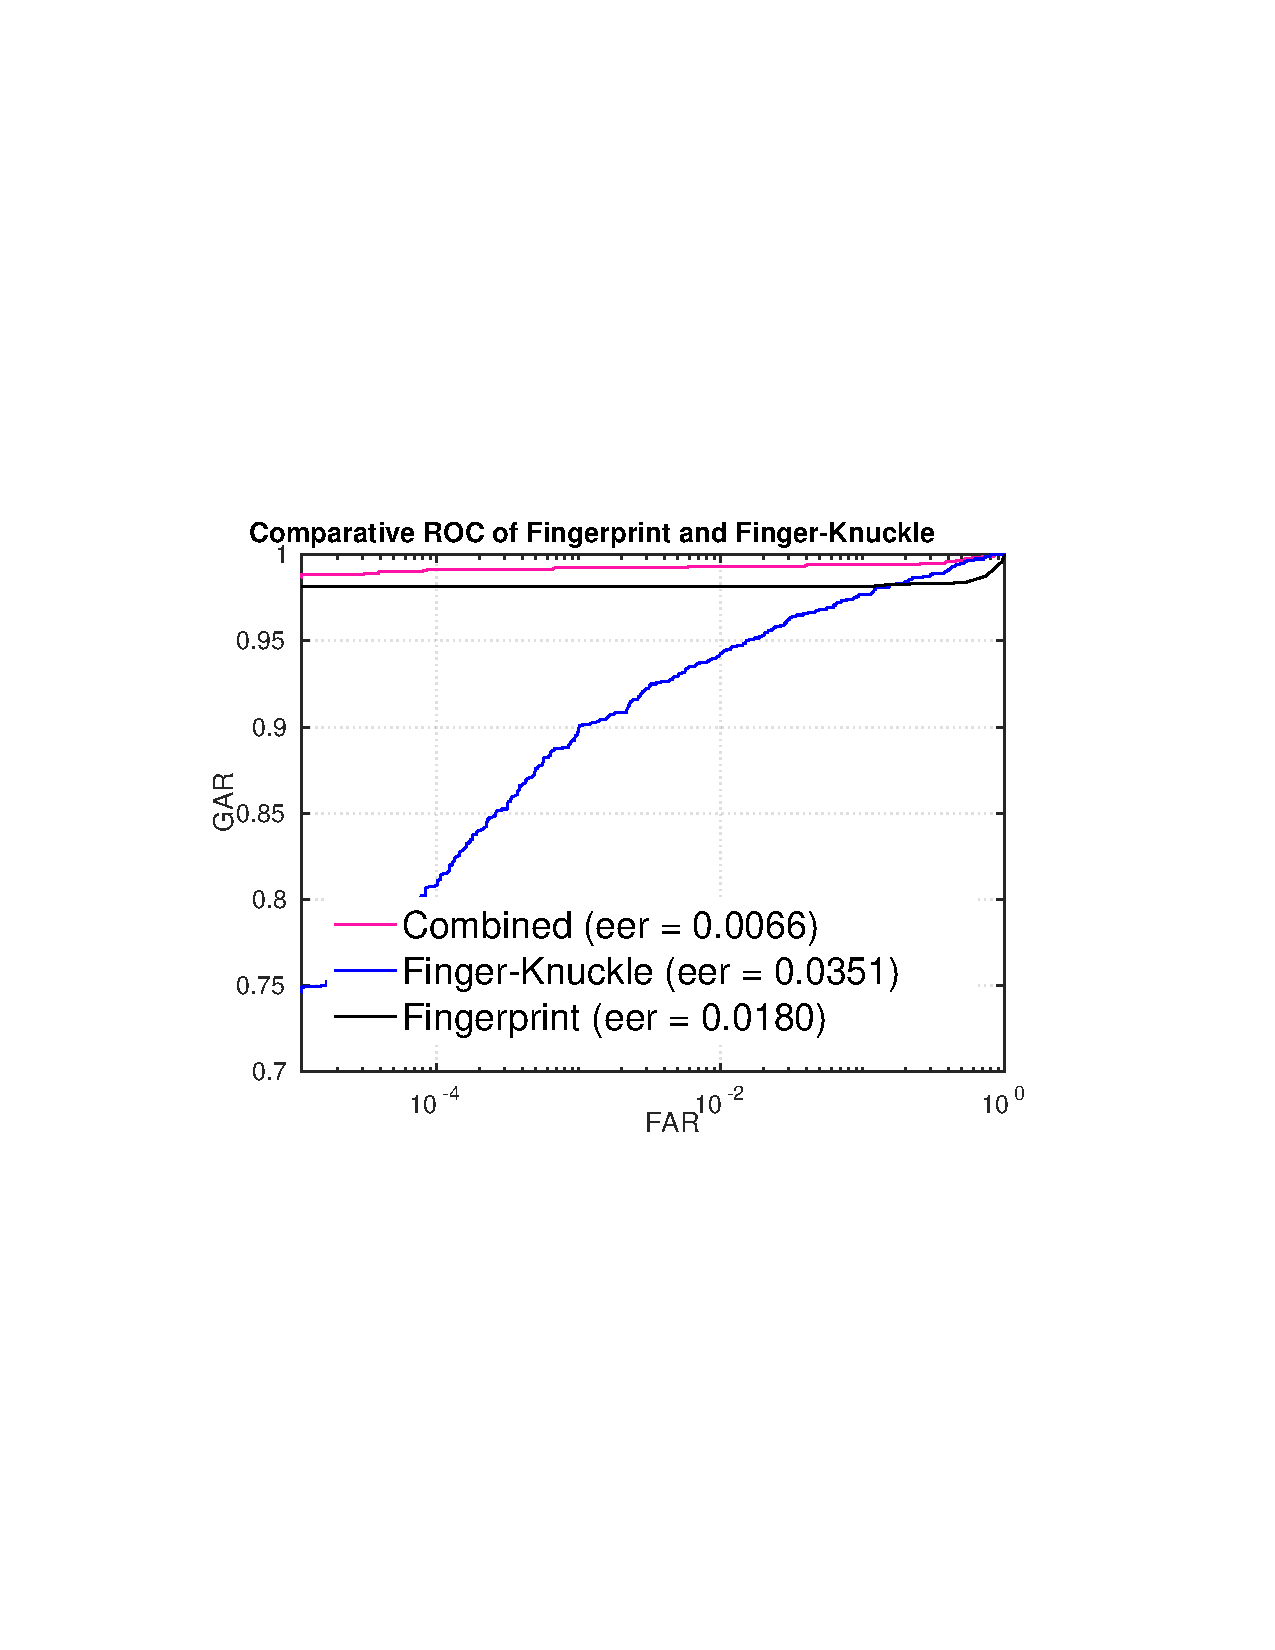
\includegraphics[width=2in]{Figures/dynamic/05.pdf}
    \label{}}
    \subfloat[]{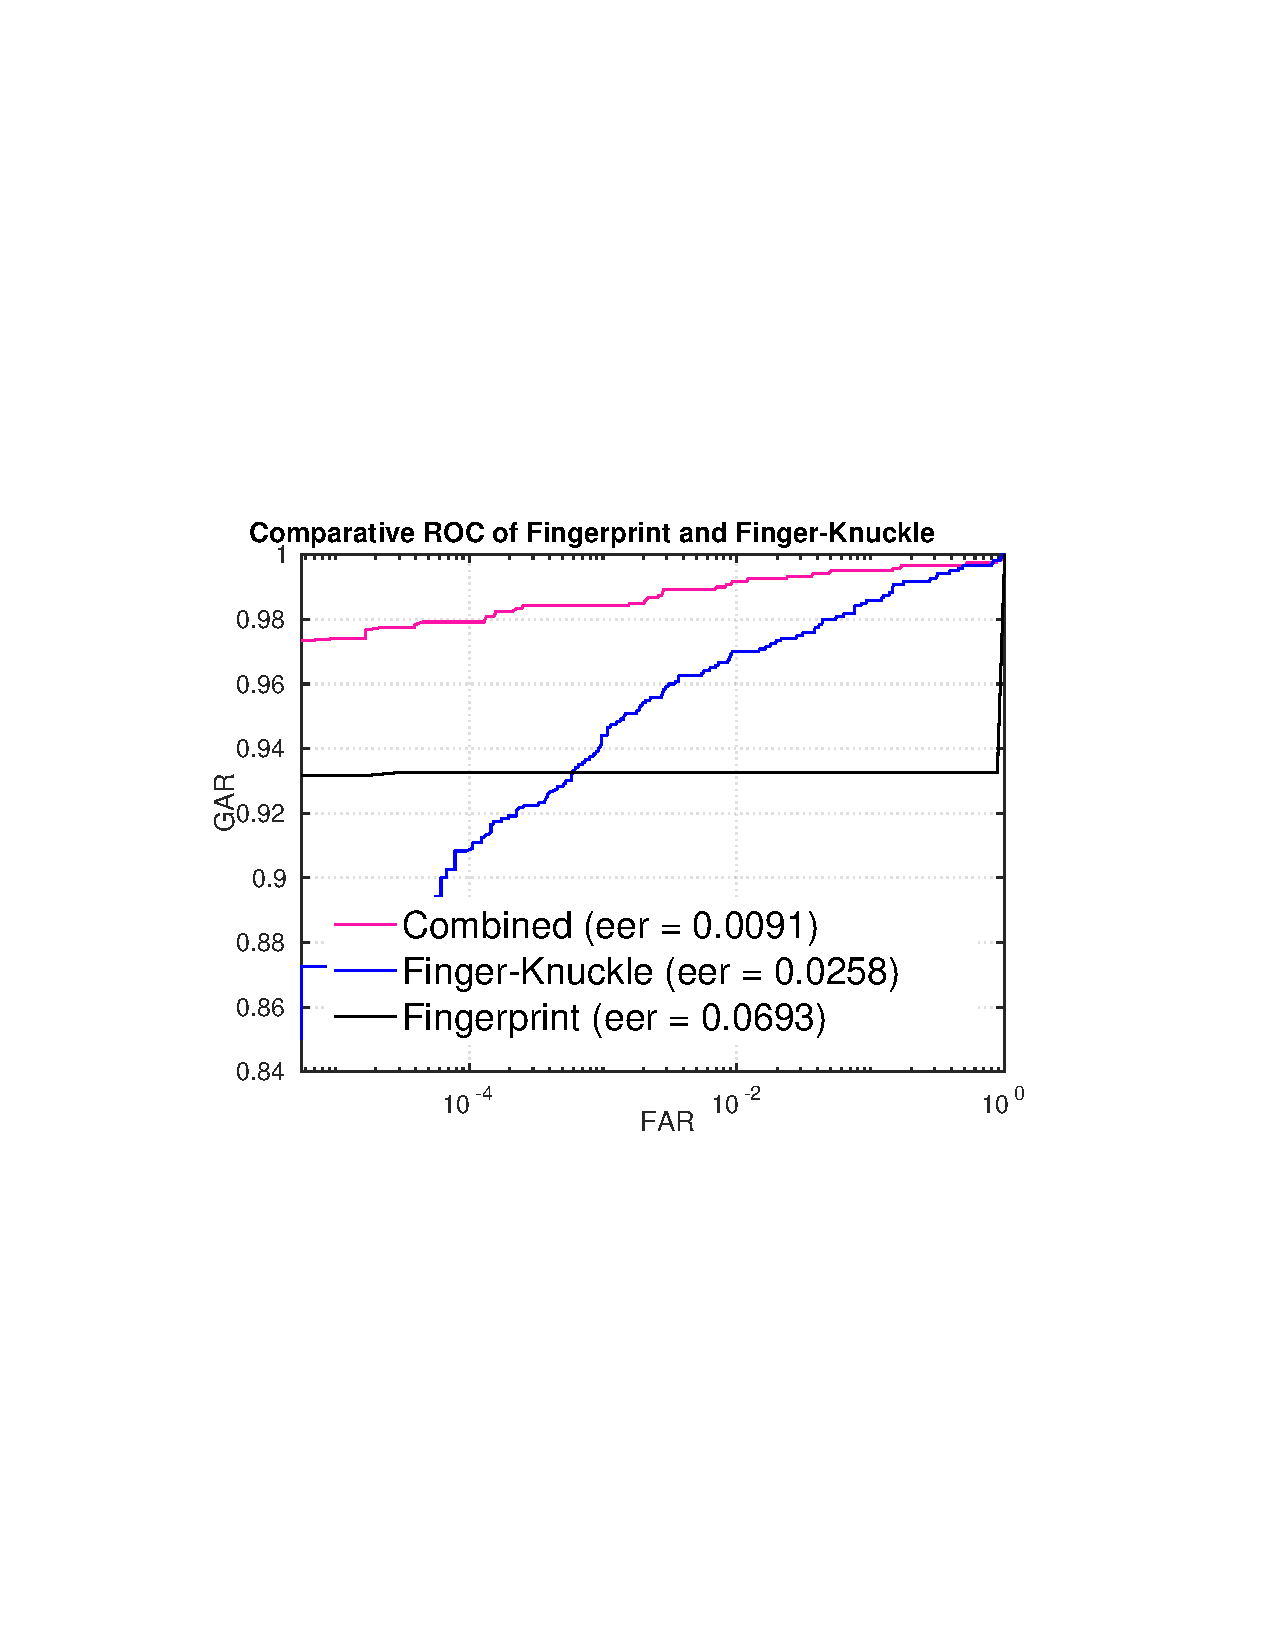
\includegraphics[width=2in]{Figures/dynamic/06.pdf}
    \label{}}
    \subfloat[]{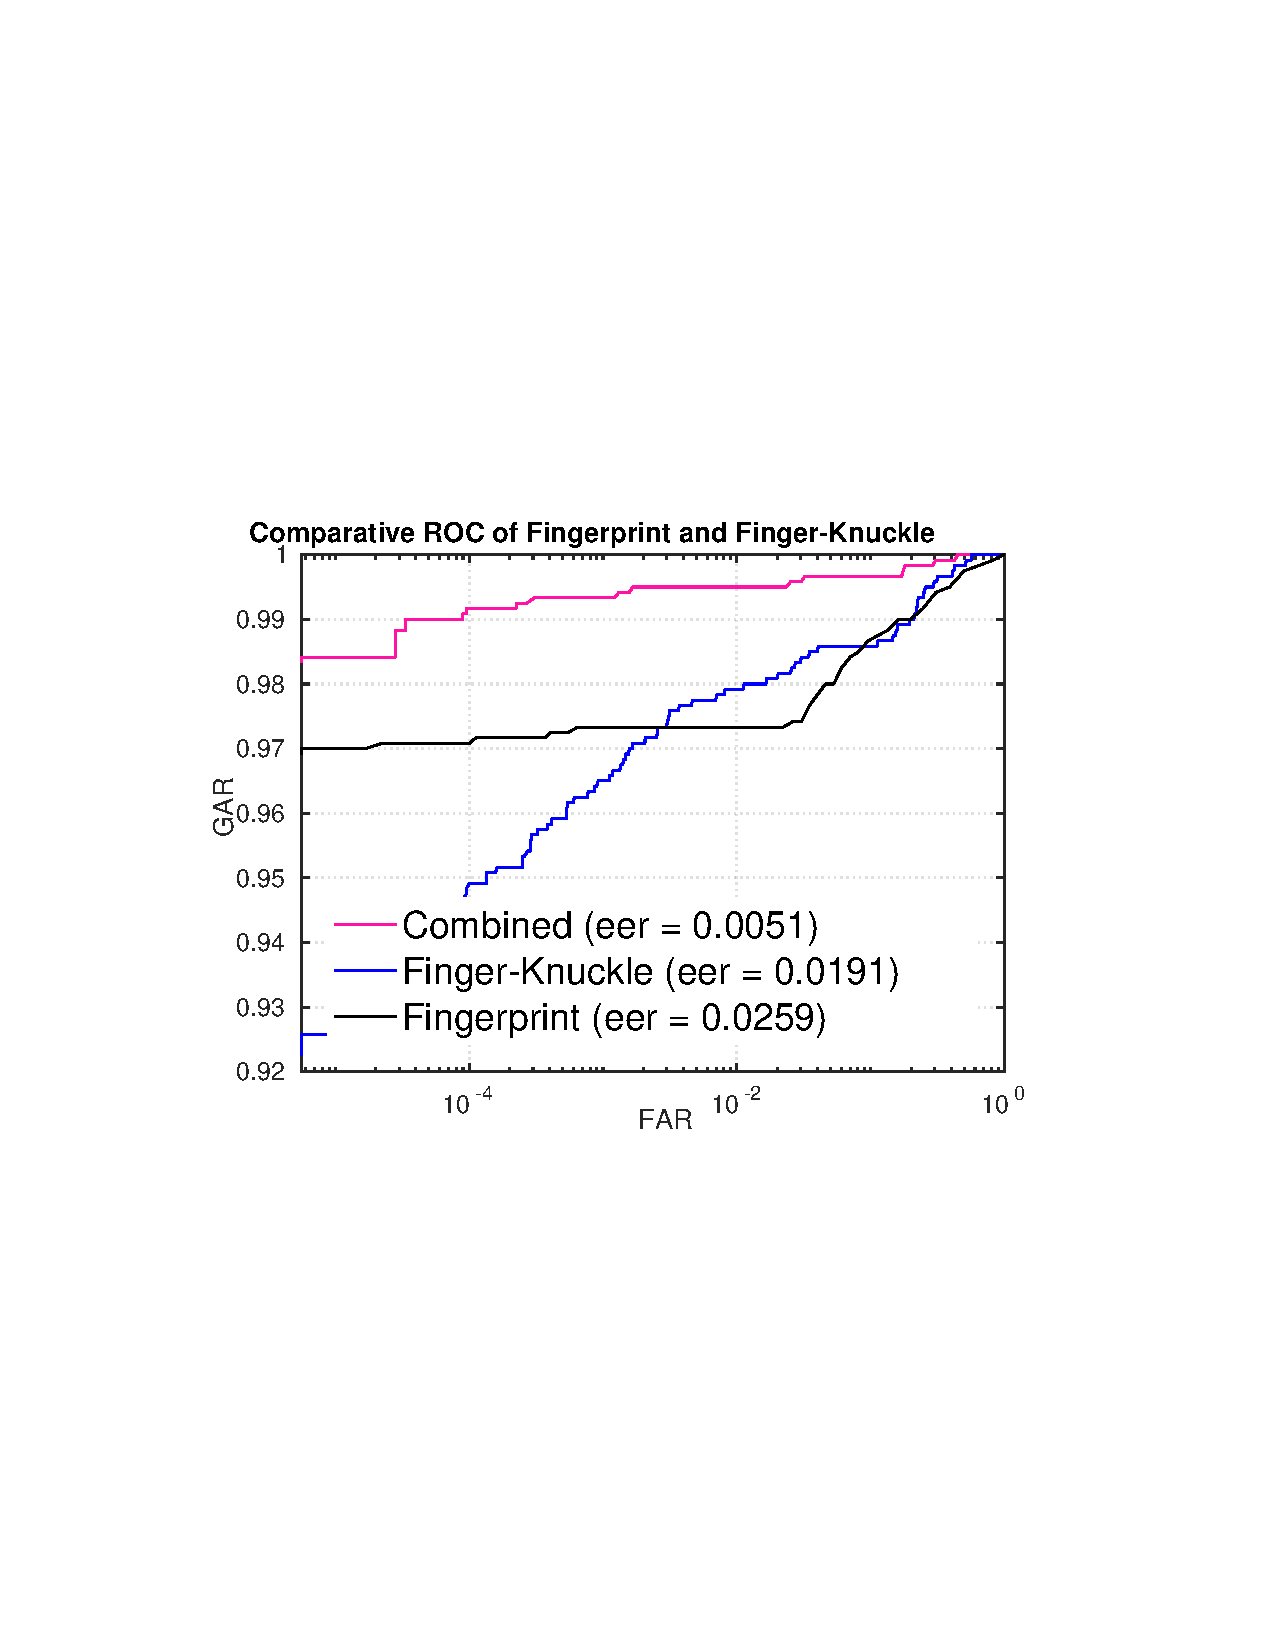
\includegraphics[width=2in]{Figures/dynamic/07.pdf}
    \label{}}

    \subfloat[]{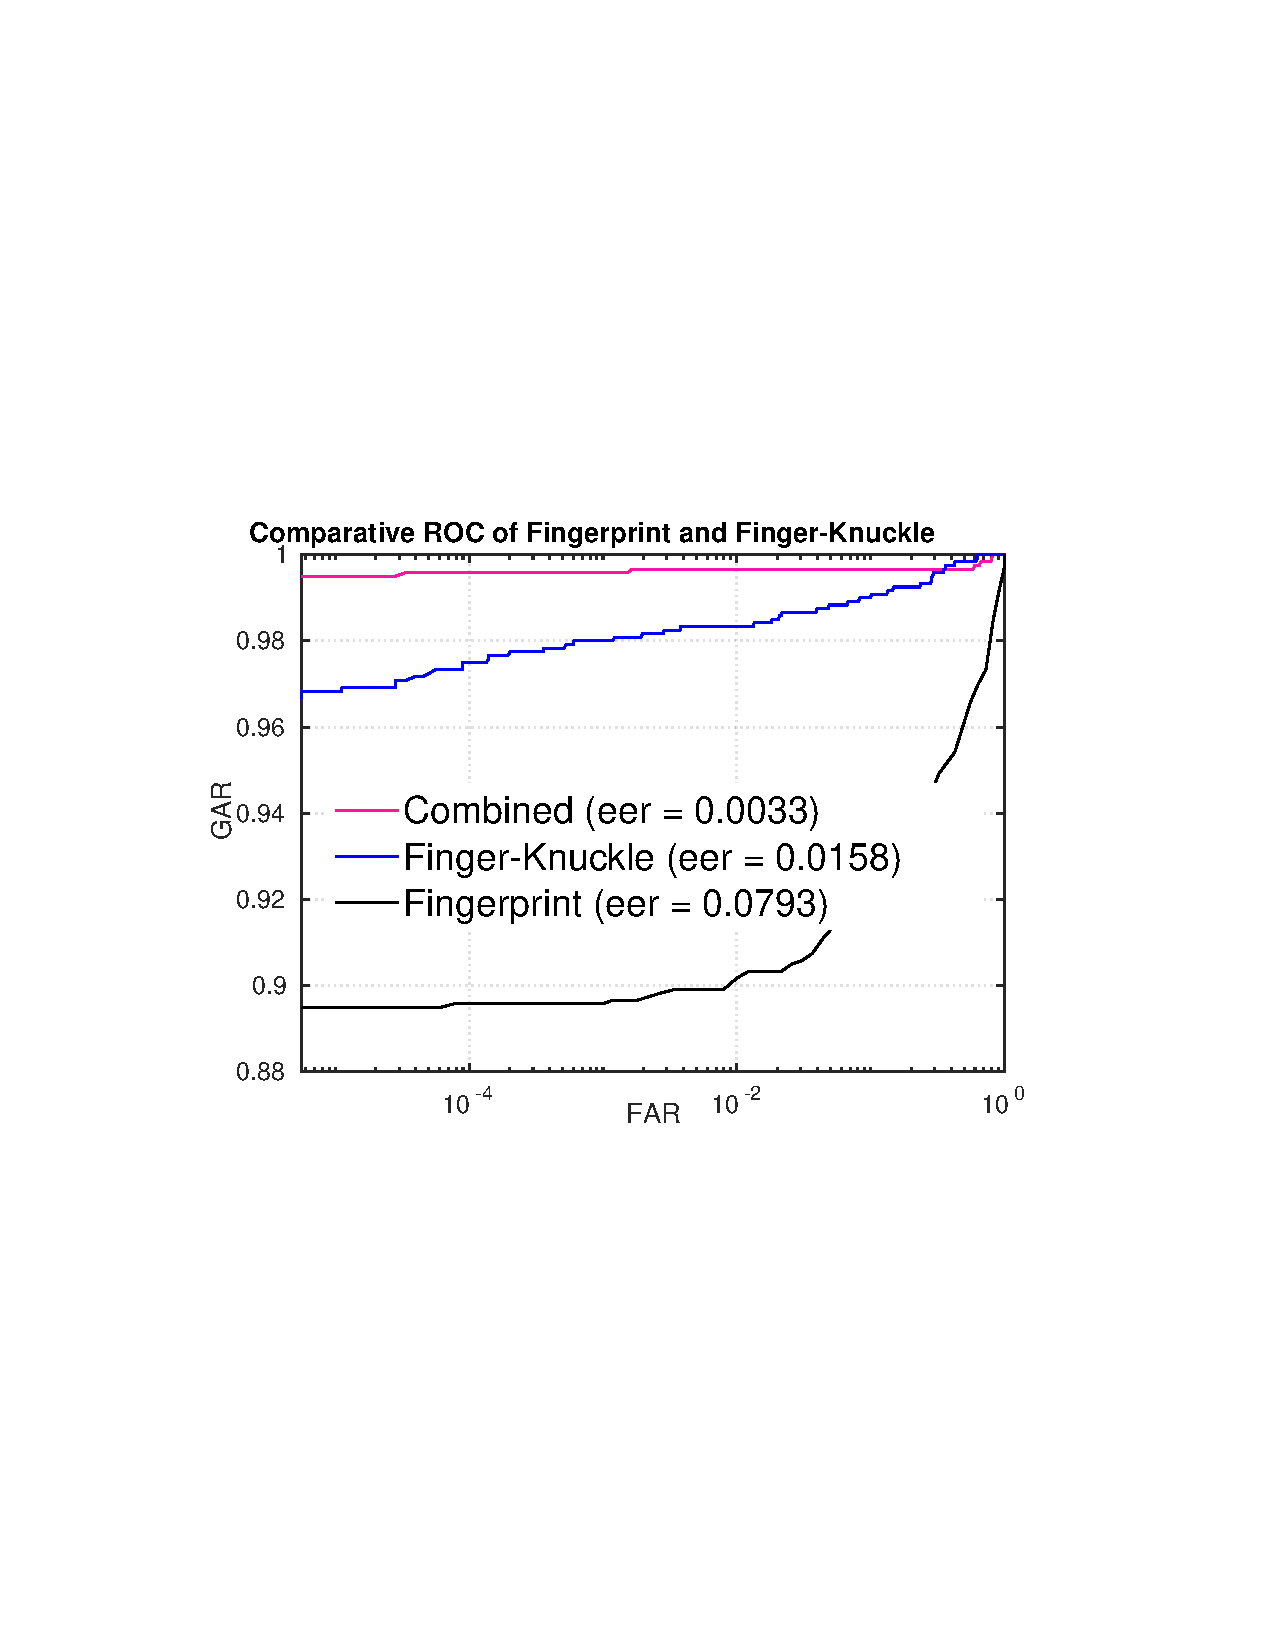
\includegraphics[width=2in]{Figures/dynamic/08.pdf}
    \label{}}
    \subfloat[]{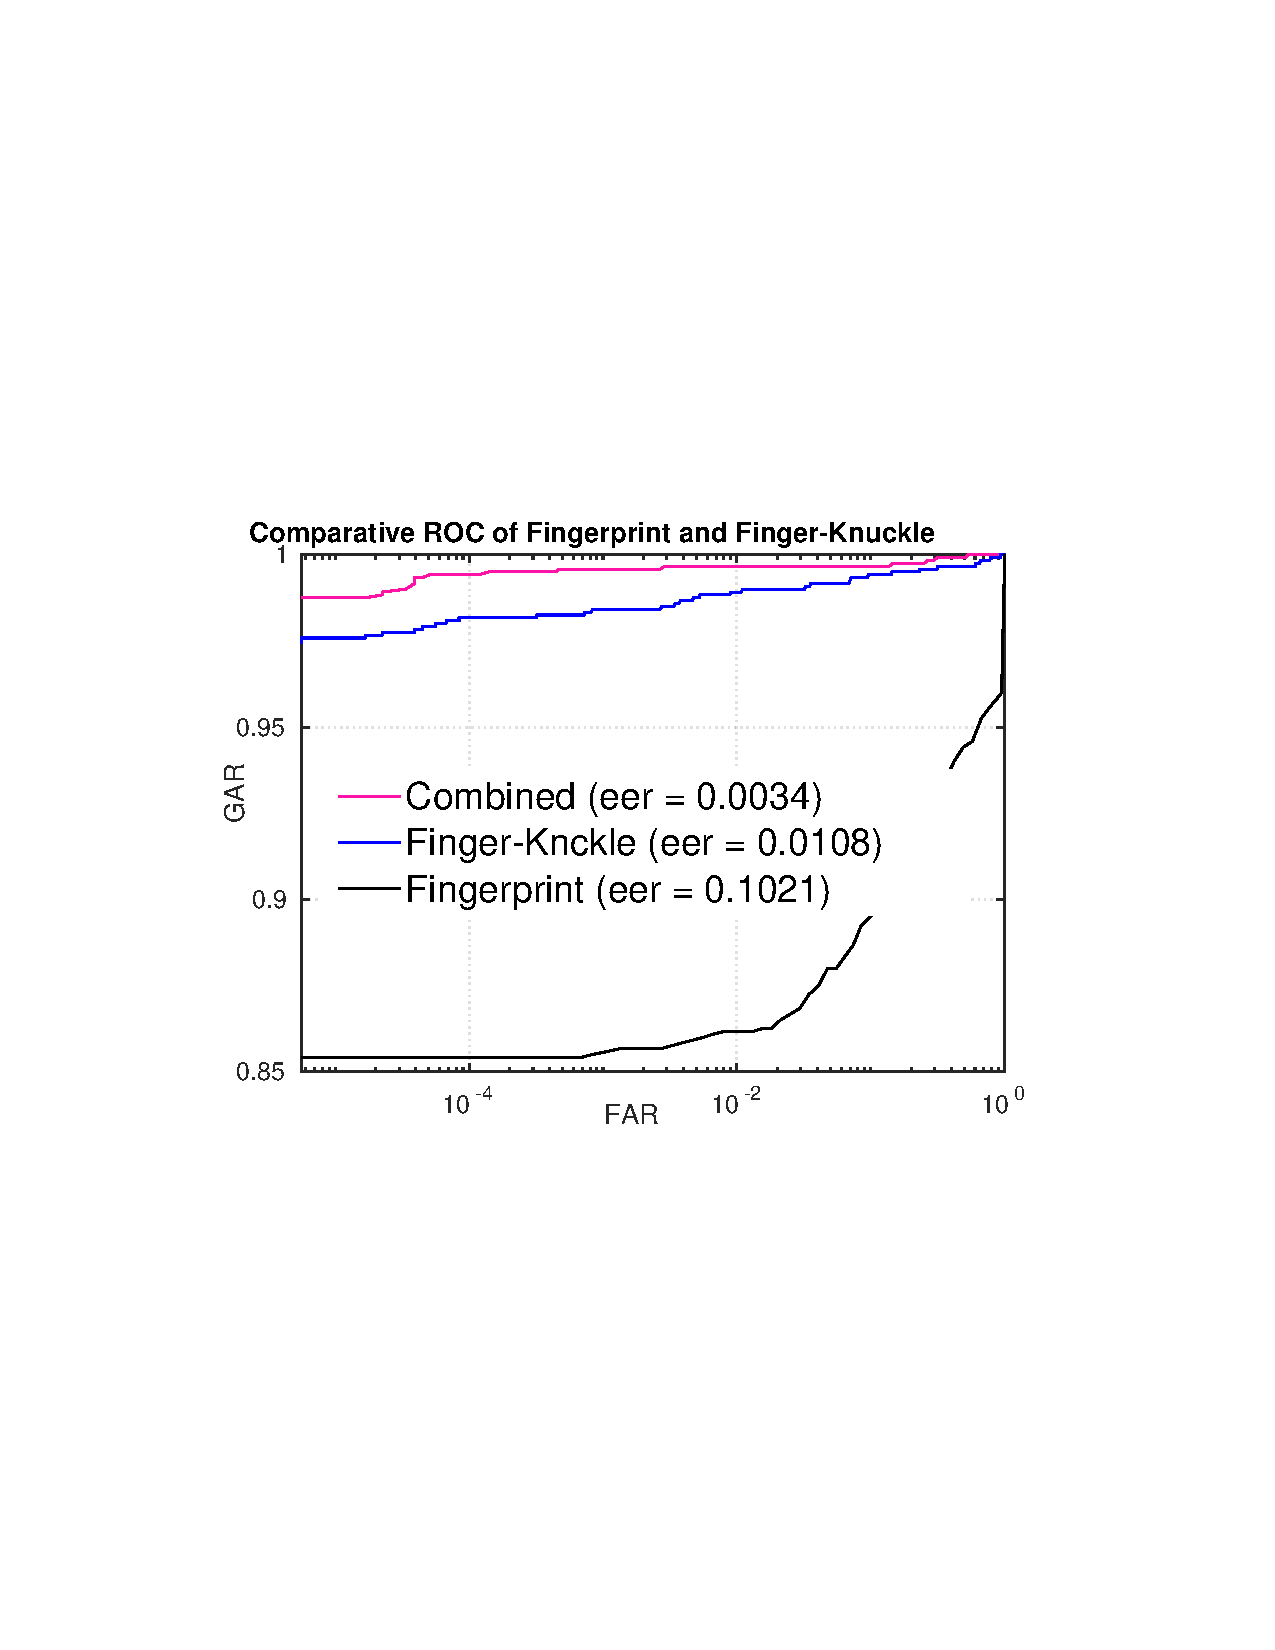
\includegraphics[width=2in]{Figures/dynamic/09.pdf}
    \label{}}
    \subfloat[]{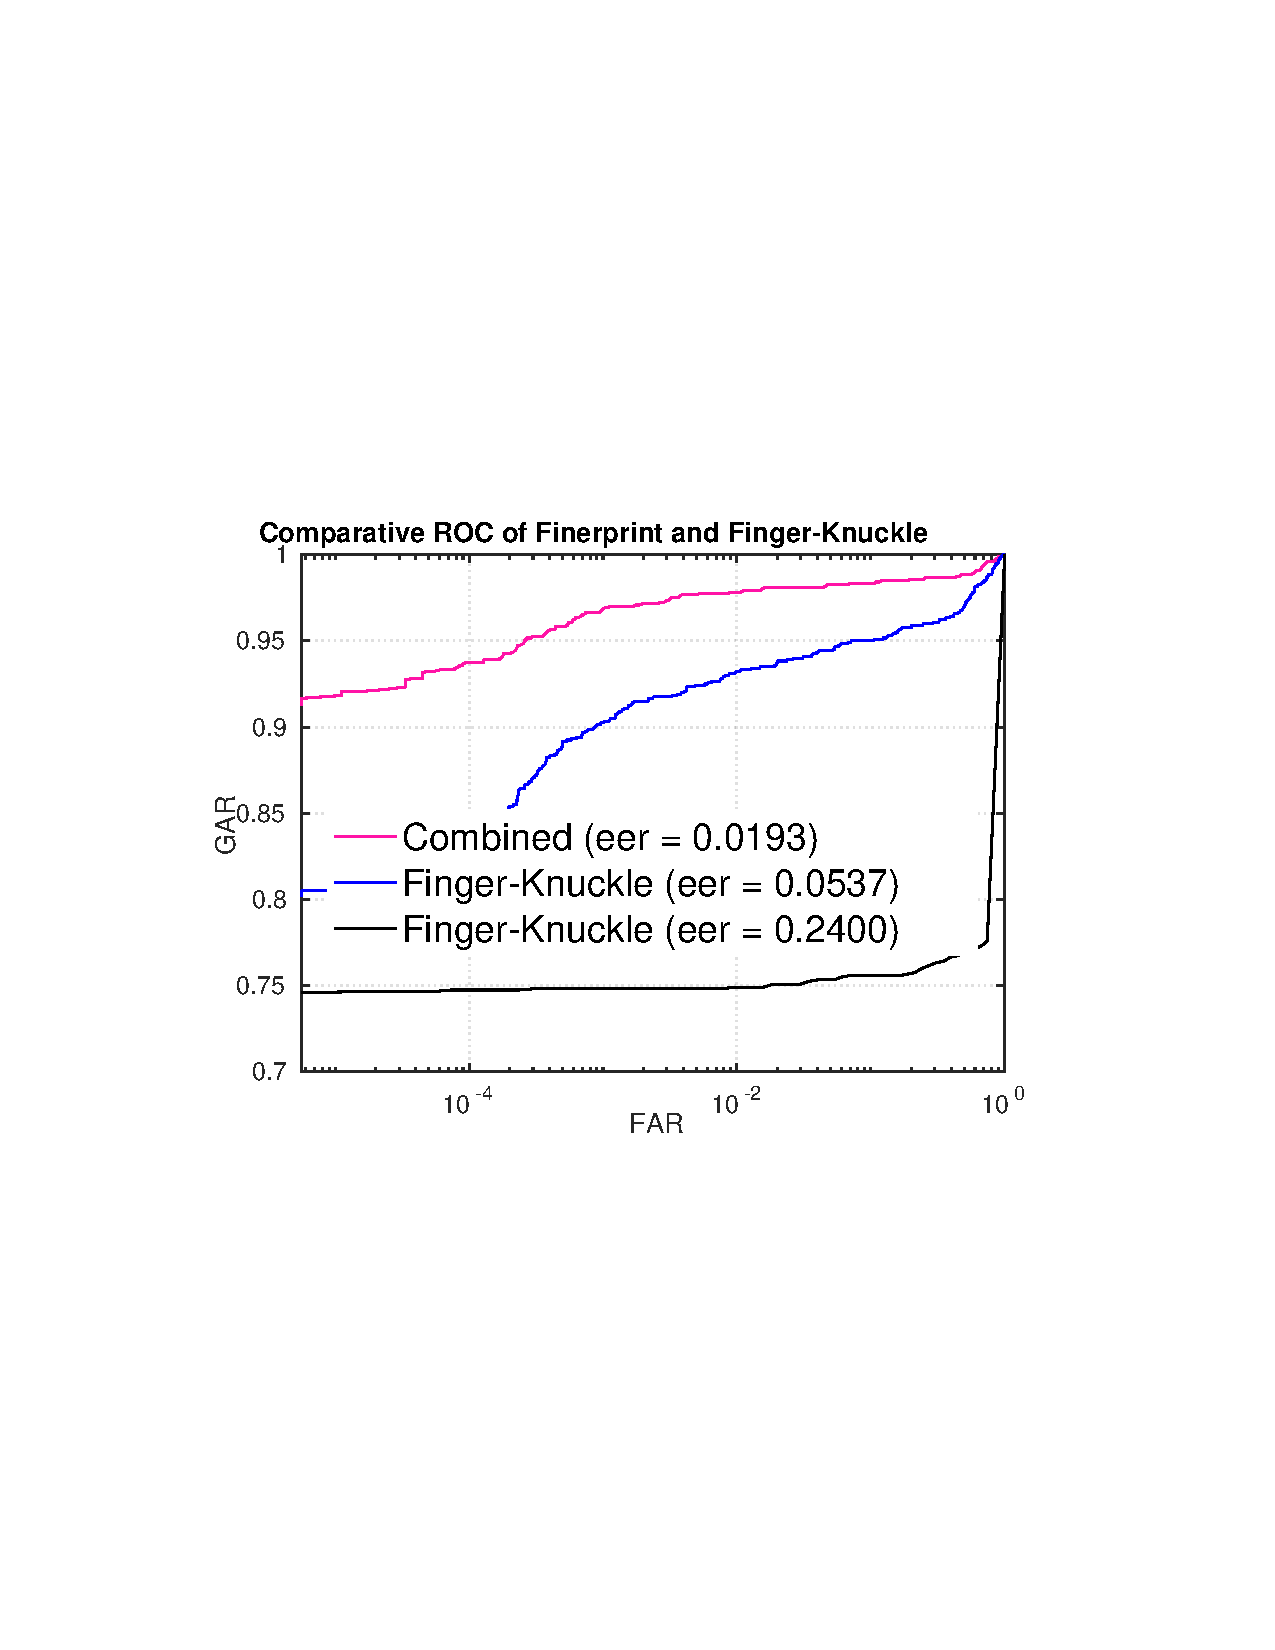
\includegraphics[width=2in]{Figures/dynamic/10.pdf}
    \label{}}
    \caption{Comparative performance the simultaneously acquired fingerprint and finger-knuckle images. The figures on the left column (a)-(e) indicate ROC from the left-hand fingers, and figures on the right column (f)-(j) indicate ROC from the right hand fingers. The figures from top to bottom row pre-sents the ROC from the little finger in (a) and (f), ring finger in (b) and (g), middle finger in (c) and (h), index finger in (d) and (i), and thumb in (f) and (j).}
    \label{joint-performance}
\end{figure*}

The combined performance from the simultaneously acquired finger knuckle and fingerprint images is shown in Figure 12. Table \ref{fusion-eer} presents a summary of respective EER values from each of the ten fingers, both individually from the finger-knuckle or fingerprint and their combination. It can be observed from these figures and table that performance improvement from the joint usage of two biometric is quite significant except for the thumbprints. The performance from the fingerprint images acquired from the thumbs is already quite high which can limit the effectiveness for simultaneously acquired finger knuckle images. The results presented in Figure 12 indicates that the extent of the performance improvement varies for the different fingers. Fig. \ref{score-distribution} illustrates the distribution of match score for the two sample fingers in our database. It can be ob-served from this figure that the distribution of match scores, from the two simultaneously acquired images, is quite distinct for the two classes. Therefore, the joint usage of such match scores is expected to offer more reliable user authentication.

\begin{table}[ht]
    \centering
    \caption{Relative EER values for the fingerprint and finger knuckle images.}
    \begin{tabular}{cccc}
    \hline
    Finger       & Finger Knuckle & Fingerprint & Combined \\ \hline
    Left Little  & 0.07491        & 0.06865     & 0.02667  \\
    Left Ring    & 0.03999        & 0.06650     & 0.01917  \\
    Left Middle  & 0.04892        & 0.08911     & 0.02167  \\
    Left Index   & 0.06746        & 0.17830     & 0.02917  \\
    Left Thumb   & 0.06493        & 0.01796     & 0.00601  \\
    Right Thumb  & 0.05334        & 0.06929     & 0.01416  \\
    Right Index  & 0.05496        & 0.02594     & 0.00916  \\
    Right Middle & 0.04922        & 0.07931     & 0.01249  \\
    Right Ring   & 0.03915        & 0.10214     & 0.01167  \\
    Right Little & 0.09746        & 0.23997     & 0.04916  \\ \hline
    \end{tabular}
    \label{fusion-eer}
\end{table}


\begin{figure}[ht]
    \begin{center}
        \subfloat[]{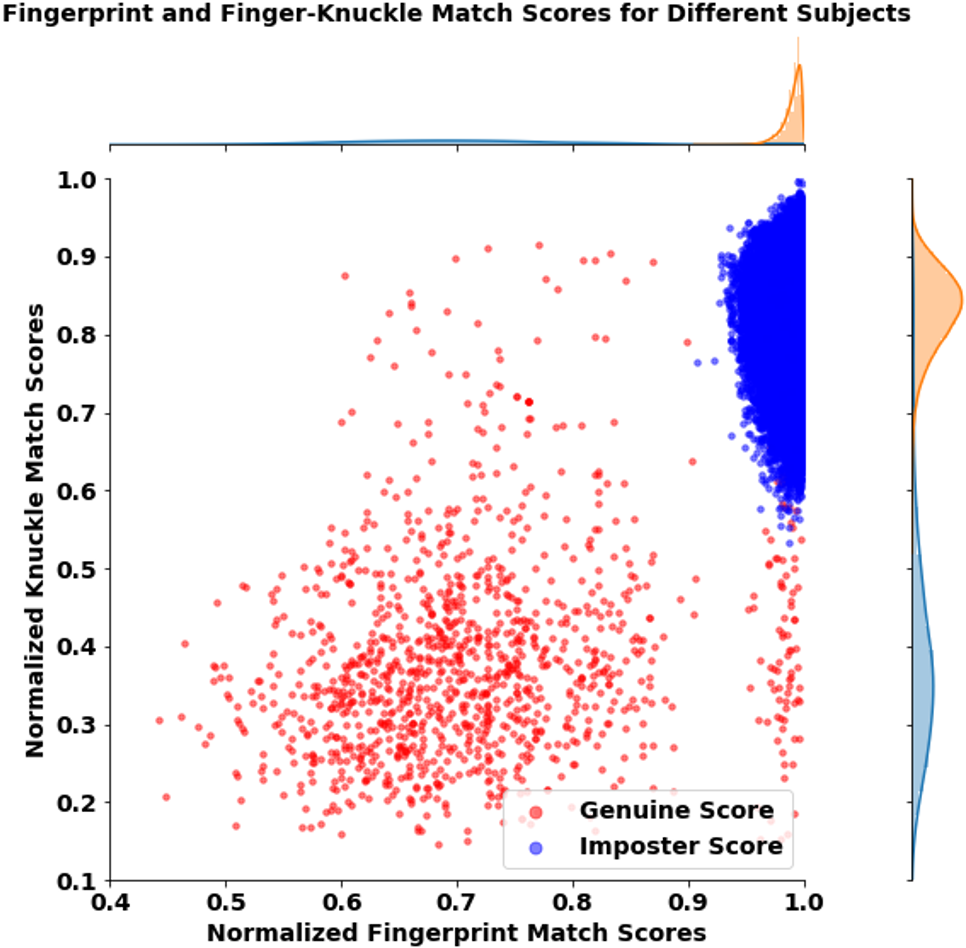
\includegraphics[width=1.65in]{Figures/score-distribution-a.png}
        \label{}}
        \subfloat[]{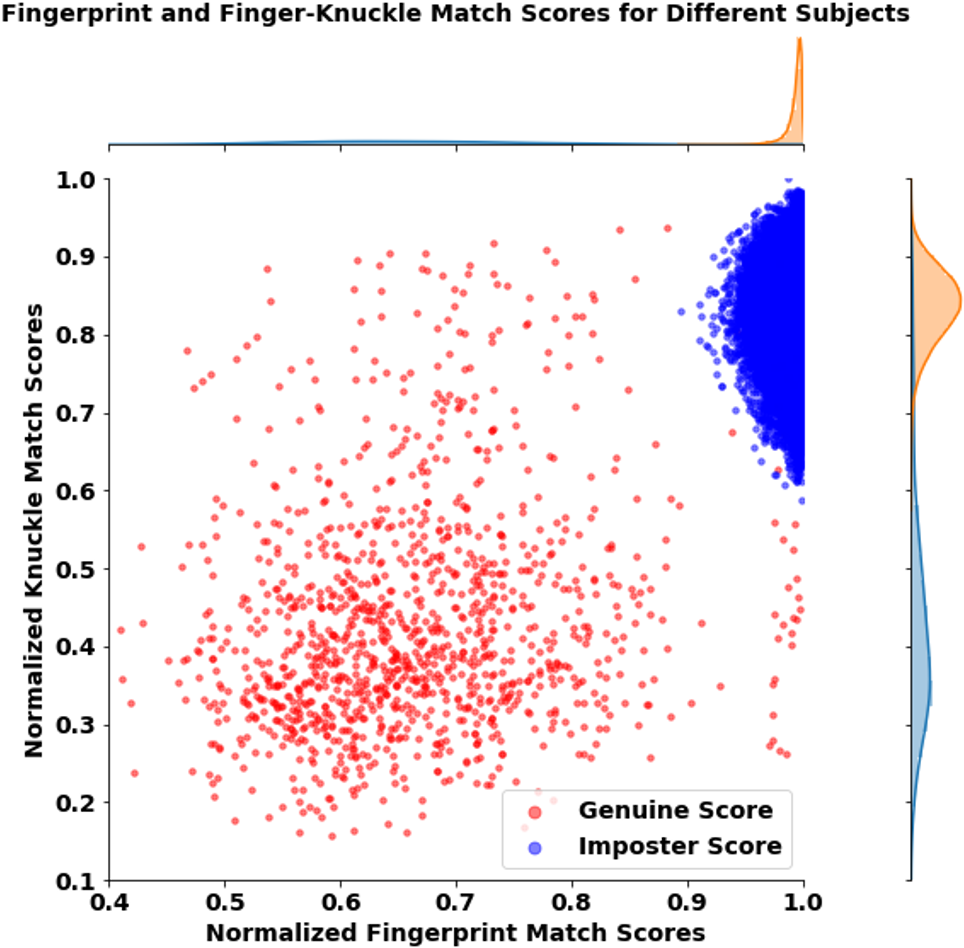
\includegraphics[width=1.65in]{Figures/score-distribution-b.png}
        \label{}}
    \end{center}
    \caption{Distribution of finger-knuckle and fingerprint match scores for two sample fingers: (a) left hand ring finger and (b) right hand index finger.}
    \label{score-distribution}
\end{figure}
\section{Discussion\label{discussion}}

\textcolor{red}{Compare finger knuckle performance with DoN, FKNet, EfficientNet, and so on.}


There are several fingerprint matching algorithms introduced in the literature \cite{maltoni2009handbook}. Among these the NBIS and MCC implementations are available in the public domain and were also attempted to ascertain the performance. Fig. \ref{compare-fingerprint} presents sample results from the comparative performance evaluation, with same test data and protocols as for the results in previous section. The performance from the COTS matcher was comparatively high and therefore this matcher was employed for all the experimental results presented in previous section. 
\begin{figure}[h]
    \centering
    \subfloat[]{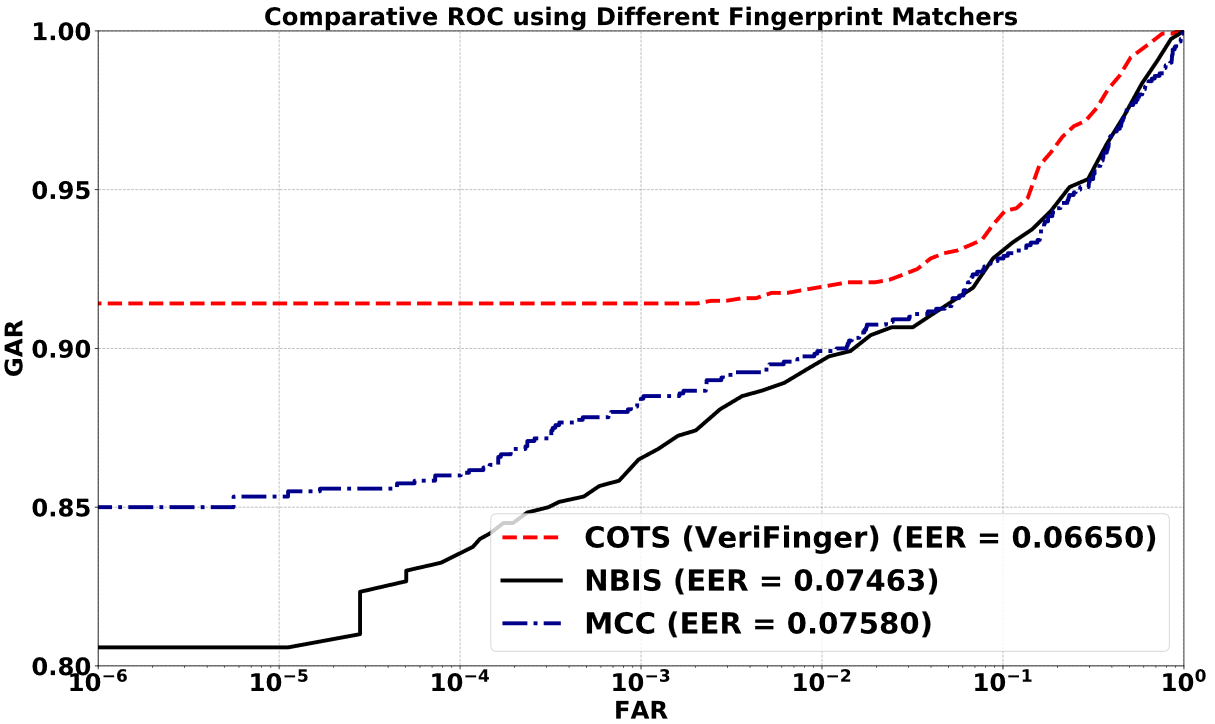
\includegraphics[width=1.6in]{Figures/compare-fingerprint-a.png}
    \label{}}
    \subfloat[]{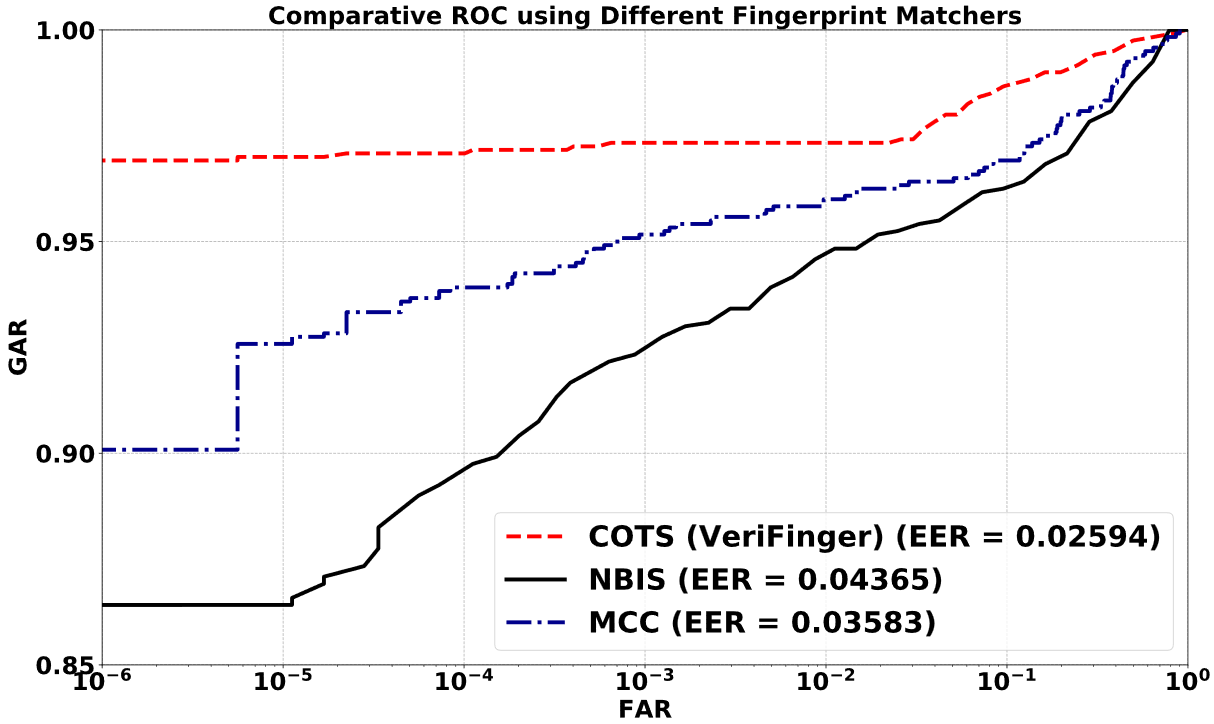
\includegraphics[width=1.6in]{Figures/compare-fingerprint-b.png}
    \label{}}
    \caption{Comparative ROC using different fingerprint matchers. (a) ROC of left ring fingerprint (b) ROC of right index fingerprint.}
    \label{compare-fingerprint}
\end{figure}

There are a range of score level combination schemes presented in the literature and can be used for the simultaneously acquired biometric samples in this work. Among these schemes, static or fixed fusion rules like sum rule, product rule, min rule, are quite attractive due to their simplicity. Therefore, we also comparatively evaluated the performance from such static score level combinations to ascertain the effectiveness of dynamic fusion introduced in this paper. Fig. \ref{compare-fusion} presents such sample comparative experimental results, with same test data and  protocols as for the results in previous section. These comparative results indicate the effectiveness of the dynamic fusion strategy to achieve more accurate performance for the simultaneously acquired fingerprint and finger knuckle images.

\begin{figure}[h]
    \centering
    \subfloat[]{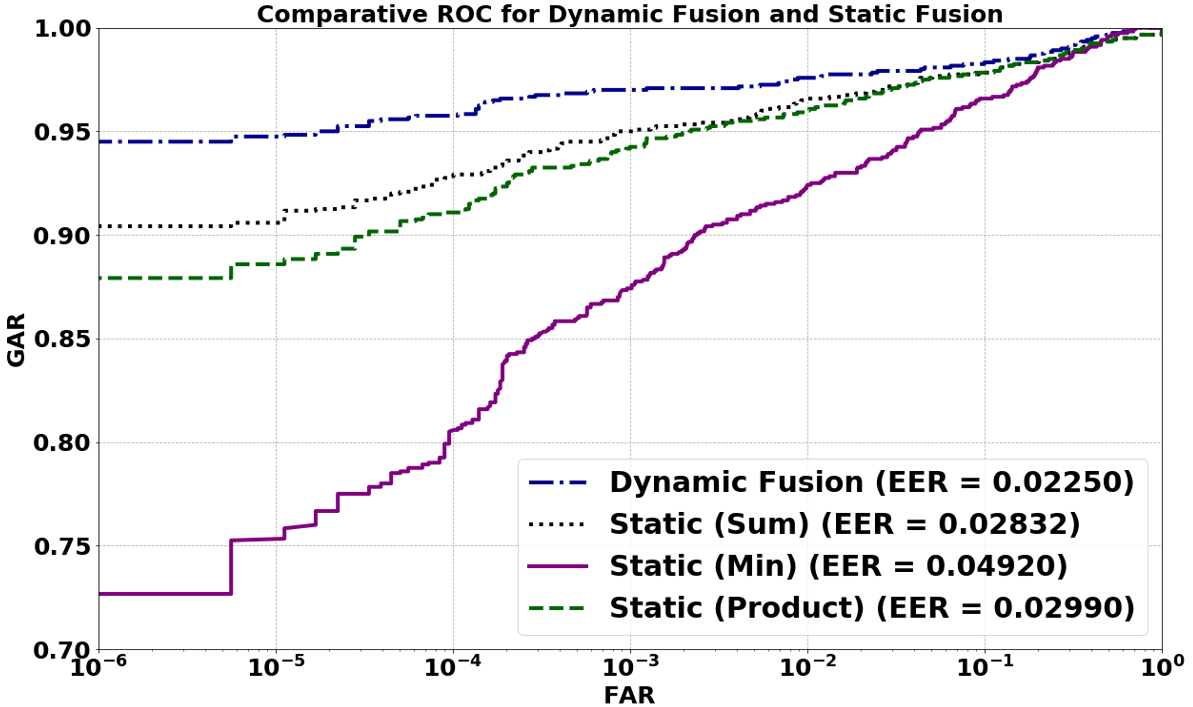
\includegraphics[width=1.6in]{Figures/compare-fusion-left.png}
    \label{}}
    \subfloat[]{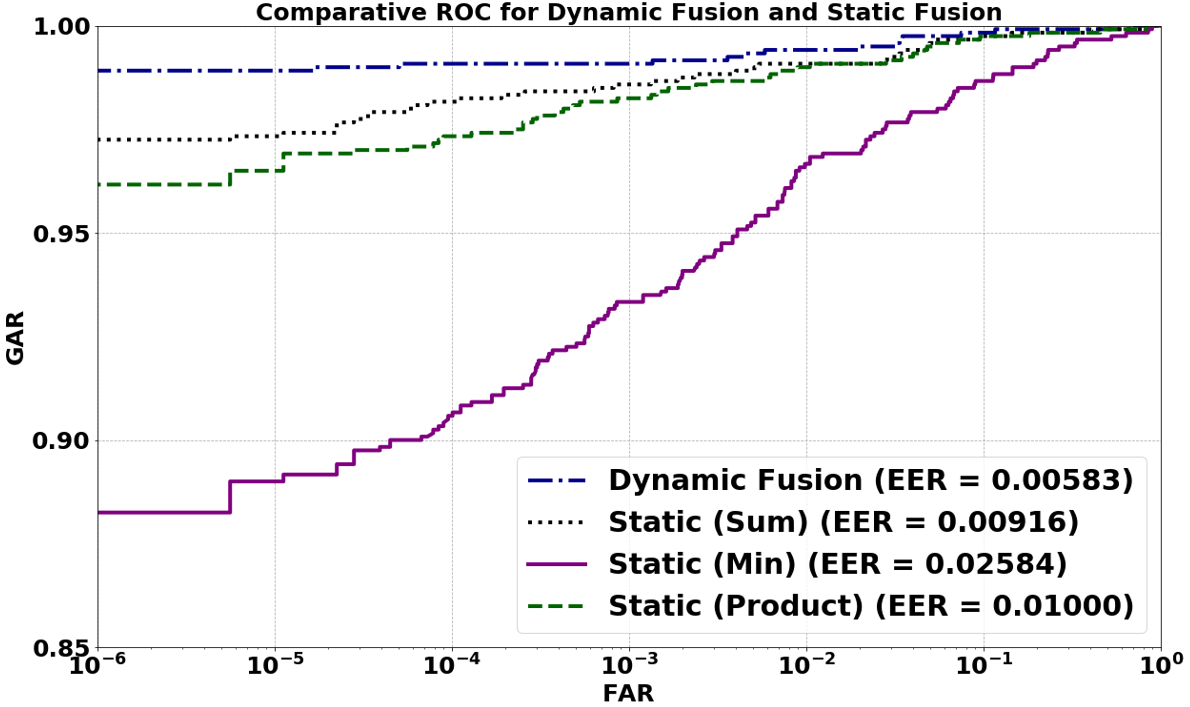
\includegraphics[width=1.6in]{Figures/compare-fusion-right.png}
    \label{}}
    \caption{Comparative ROC using different fingerprint matchers. (a) ROC of left ring fingerprint (b) ROC of right index fingerprint.}
    \label{compare-fusion}
\end{figure}

\begin{figure}[h]
    \begin{center}
    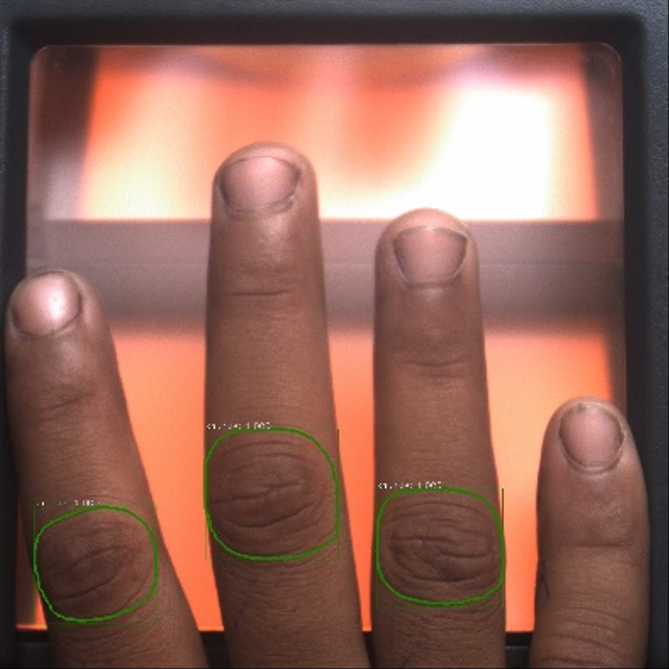
\includegraphics[width=1.1in]{Figures/failure-a.png}
    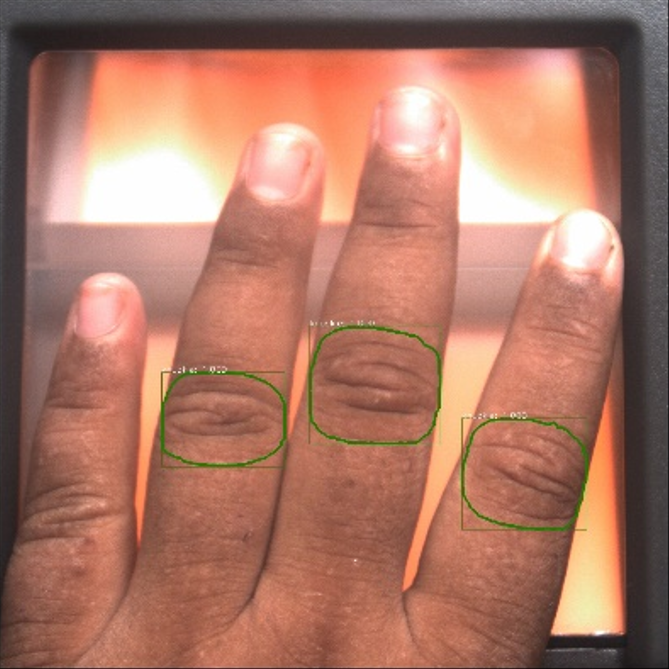
\includegraphics[width=1.1in]{Figures/failure-b.png}
    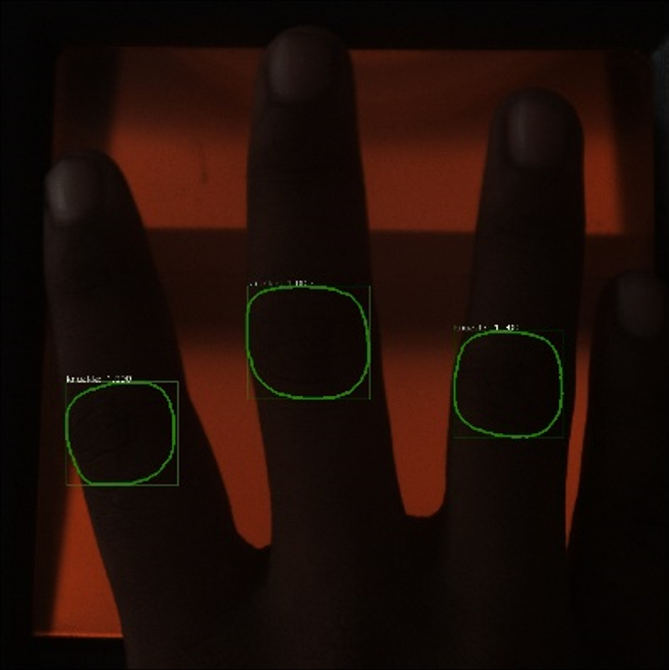
\includegraphics[width=1.1in]{Figures/failure-c.png}
    
    \hspace{0.001in}
    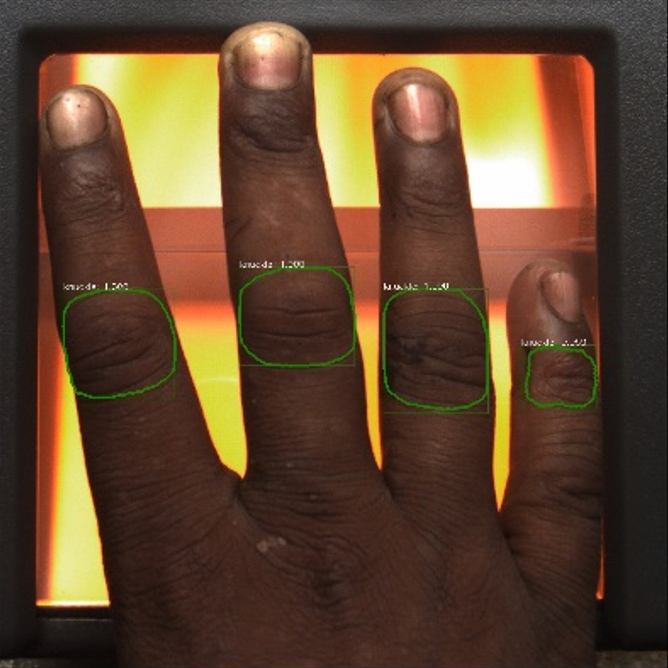
\includegraphics[width=1.1in]{Figures/failure-d.png}
    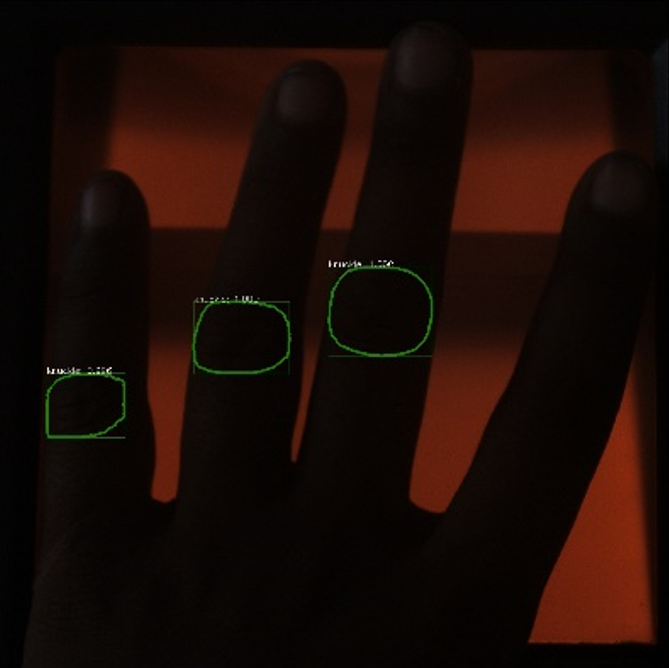
\includegraphics[width=1.1in]{Figures/failure-e.png}
    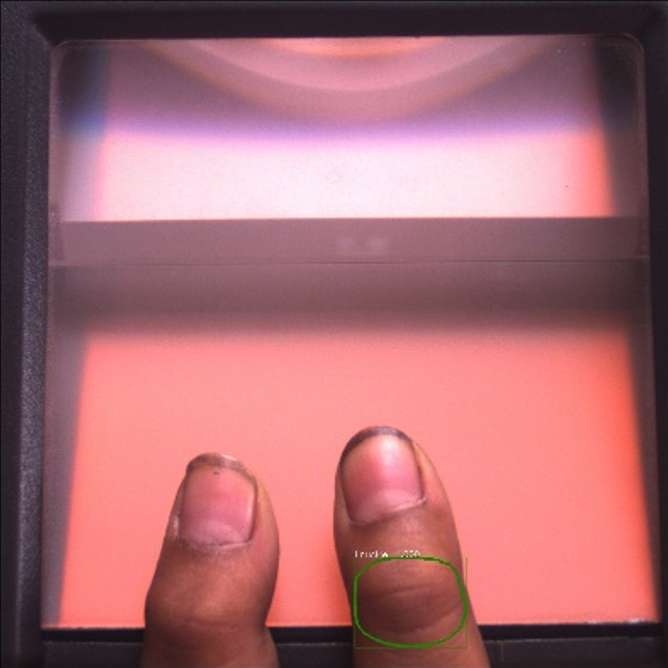
\includegraphics[width=1.1in]{Figures/failure-f.png}
    \caption{Image samples illustrating failure cases for the finger knuckle detection.}
    \label{failure-case}
    \end{center}
\end{figure}


The experimental results presented in previous section indicated the effectiveness of the simultaneously acquired finger knuckle images for the user authentication. Despite our efforts and the limited\footnote[2]{The images used to train the detector were acquired from different users and none of these subjects’ images were used for the performance evaluation presented in Section \ref{experiment}.}  availability of the images, there are many cases where the detector fails to detect the finger knuckle regions. Fig. \ref{failure-case} shows such sample failure cases for the finger knuckle detection. The first image on the left in this figure illustrates that only three finger knuckle regions are detected while the detection of finger knuckle from the little finger is not successful. The image sample in the middle indicates that the detection of finger knuckle from the left little finger is influenced by the pose of the presented finger that covers dark background of the slap fingerprint sensor. The image samples on the right side in this figure illustrates the samples that are acquired under adverse environment where the successful detection of most finger knuckle is quite encouraging. How-ever, there are still some failure cases for the accurate detection. Such failure can be attributed not just to the availability of very limited training images but also to the limitations from the images where only partial finger knuckle regions are visible due to the presentation or the pose of presented fingers.  In many cases the knuckle regions from the thumbs are either partially imaged or not detected (e.g. last image sample in Fig. \ref{failure-fingerprint}). This is the key reason that the performance from the such finger knuckle regions is relatively low while the corresponding fingerprint performance is very high. Therefore, a separate scheme to further improve the overall match accuracy, on much larger databases as for the real applications, is required and is suggested in the further extension of this work.  

\begin{figure}
    \begin{center}
        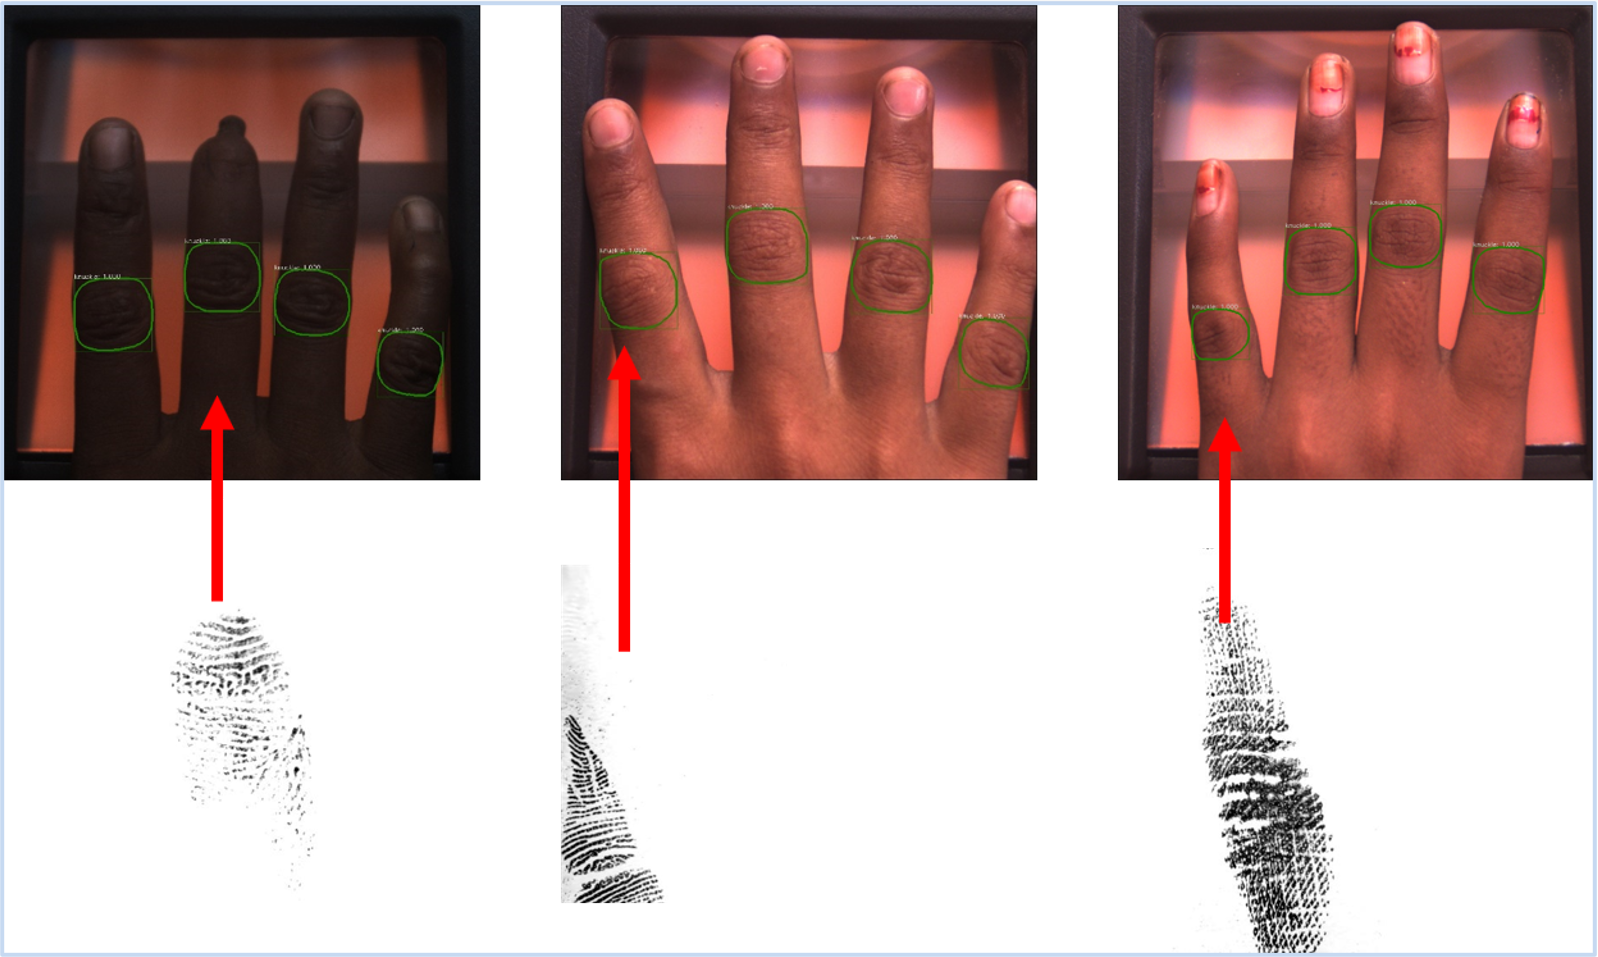
\includegraphics[width=3in]{Figures/failure-fingerprint.png}
    \end{center}
    \caption{Image samples illustrating failure cases for the fingerprint detection.}
    \label{failure-fingerprint}
\end{figure}

The fingerprint detection and the segmentation algorithms are quite matured and most commercial slap fingerprint sensors provide such implementations along with the sensor drivers. The quality of detected and segmented fingerprint images can also vary and especially for the fingerprint acquired during the real applications. These limitations were also observed during this work and there are many cases where the finger-print region is not detected or detected images are of quite low quality. The images in Fig. \ref{failure-fingerprint} presents such failure cases for the acquired fingerprint images. The images on the first row are included to indicate the presentation of the volunteers on the slap fingerprint sensor.  The images shown in this figure on the second row illustrates the correspondingly segmented fingerprint images. The leftmost segmented image sample in this figure indicates that the middle finger fingerprint is incorrectly detected or segmented as this user has some inherent challenges with his/her fingertip. The second sample from the left indicates \textit{partial} index fingerprint segmentation and this can be largely due to the presentation of index finger which is not completely within the marked sensor surface.  Similarly, the rightmost fingerprint image sample in this figure indicated segmented fingerprint images are degraded and this can be attributed to the limitations with the pressure or the presentation fingers on the sensor surface. 
\section{Conclusion and Further Work\label{conclusion}}

This paper introduces a new biometric system that can simultaneously acquire finger knuckle and fingerprint images, using the existing or widely deployed slap fingerprint devices, for more reliable user identification. We introduced a completely automated approach to reliably segment individual finger knuckle regions from the slap finger-print dorsal images with multiple fingers. More importantly, we developed a new database from such simultaneously acquired finger knuckle and fingerprint images using 4-4-2 protocols and provide \cite{datalink} the entire database to advance further research in this area. One of the key advantages of this system lies in its simplicity, as the finger-knuckle images are acquired using an additional or low-cost camera under the ambient illumination. Therefore, this system can be added to the existing or deployed slap-fingerprint devices at the border-crossings with the least inconvenience or the cost.    

The work detailed in this paper should be considered as the first attempt and further work is required to address the limitations. Firstly, our emphasis has been on simplicity and therefore a simplified dynamic fusion scheme was used to consolidate match scores from the simultaneously acquired biometric. More complex and dynamic fusion schemes that can also consider biometric image quality are expected to further improve the performance and are suggested for the further work. Secondly, the performance from the finger-knuckle detector needs improvement, especially for the thumb images. This can be attempted by using changing the detector backbone from mask RCNN to other detector \cite{redmon2016you} and enhancing the number/variety of training samples. Finally, this is first such attempt and therefore database from 120 volunteers could be acquired and none of these were paid or received any honorarium. A large-scale database from thousands of subjects is required to more effectively ascertain the performance improvement. In this work we only presented the performance improvement from the combination of two simultaneously acquired biometric for the individual fingers as the combination of all fingers can achieve full accuracy on relatively small user population. Therefore availability of large scale database can validate the effectiveness of performance improvement for a range of deployments applications which generally have millions of users for the identification.

\bibliography{references.bib}
\bibliographystyle{unsrt}


\end{document}


